\documentclass[12pt,a4paper]{article}

\usepackage{array}
\usepackage{geometry}
\usepackage{graphicx}
\usepackage{fancyhdr}
\usepackage{amsmath}
\usepackage{amsfonts}
\usepackage{amssymb}
\usepackage{color}
\usepackage{hyperref}
\usepackage{tikz}
\usetikzlibrary{shapes.geometric,arrows,positioning,shadows}
\usepackage{pgfgantt}
\usepackage{float}
\usepackage{listings}
\usepackage{xcolor}
\usepackage{booktabs}
\usepackage{multirow}
\usepackage{subcaption}
\usepackage{titlesec}
\usepackage{multicol}
\usepackage{caption}
\usepackage{colortbl}
\usepackage{geometry}



% Remove colour styling that causes table issues
\captionsetup{
    font={bf,small},
    textfont={color=bodytext},
    labelfont={color=primaryblue, bf},
    justification=centering,
    singlelinecheck=false,
    labelsep=period,
    skip=10pt,
    position=bottom
}

% Professional subcaption formatting – coordinated styling
\captionsetup[sub]{
    font={bf,footnotesize},
    textfont={color=bodytext},
    labelfont={color=secondaryblue, bf},
    justification=centering,
    singlelinecheck=false,
    labelsep=period,
    skip=8pt
}

% Professional table formatting with coordinated styling
\definecolor{tableheader}{RGB}{0,82,165}         % Primary blue for headers
\definecolor{headercolor}{RGB}{0,82,165}         % Alias for compatibility
\definecolor{tablebody}{RGB}{240,248,255}        % Very light blue
\definecolor{tableaccent}{RGB}{25,118,210}       % Secondary blue accent
\definecolor{tableborder}{RGB}{0,82,165}         % Primary blue border

% Additional colour definitions for enhanced tables
\definecolor{headertext}{RGB}{255,255,255}       % White text for headers
\definecolor{bodytext}{RGB}{66,66,66}            % Professional dark gray
\definecolor{tablealt1}{RGB}{248,251,255}        % Alternating row colour 1
\definecolor{tablealt2}{RGB}{235,245,251}        % Alternating row colour 2
\definecolor{greentable}{RGB}{76,175,80}         % Professional green
\definecolor{orangetable}{RGB}{255,152,0}        % Professional orange
\definecolor{purpletable}{RGB}{156,39,176}       % Professional purple

% Enhanced table styling commands
\newcommand{\tableheaderrow}[1]{\rowcolor{tableheader}\textcolor{headertext}{\textbf{#1}}}
\newcommand{\tablealtrow}{\rowcolor{tablealt1}}
\newcommand{\tablealtrowtwo}{\rowcolor{tablealt2}}
\newcommand{\specialheader}[2]{\rowcolor{#1}\textcolor{headertext}{\textbf{#2}}}
\renewcommand{\contentsname}{\textcolor{primaryblue}{Table of Contents}}

% Set default array rule width for professional borders
\setlength{\arrayrulewidth}{1.2pt}

% Configure hyperref with professional colours
\hypersetup{
    colorlinks=true,
    linkcolor=primaryblue,
    filecolor=secondaryblue,      
    urlcolor=accentblue,
    pdftitle={System Analysis of Tech Rajshahi Ltd},
    pdfauthor={Nazifa Tasnim Shifa, Chandan Biswas, Md. Ahsanul Karim (Abir), Suraiya Jahan, Sifat Ullah},
    pdfsubject={Systems Analysis and Design Lab Report}
}

% Enhanced code listings with professional colours
\lstset{
    basicstyle=\ttfamily\footnotesize,
    backgroundcolor=\color{lightgray},
    frame=leftline,
    framerule=3pt,
    rulecolor=\color{primaryblue},
    breaklines=true,
    captionpos=b,
    numbers=left,
    numberstyle=\tiny\color{darkgray}\bfseries,
    stepnumber=1,
    numbersep=12pt,
    keywordstyle=\color{primaryblue}\bfseries,
    commentstyle=\color{mediumgray}\itshape,
    stringstyle=\color{secondaryblue},
    emphstyle=\color{accentblue}\bfseries,
    showstringspaces=false,
    tabsize=2,
    xleftmargin=20pt,
    framexleftmargin=15pt,
    numberbychapter=false,
    firstnumber=1
}

% ===================== PROFESSIONAL COLOUR SCHEME =====================
% Define professional colour palette
\definecolor{primaryblue}{RGB}{0,82,165}        % Deep professional blue
\definecolor{secondaryblue}{RGB}{25,118,210}    % Medium blue
\definecolor{accentblue}{RGB}{100,181,246}      % Light blue accent
\definecolor{lightblue}{RGB}{173,216,230}       % Light blue for backgrounds
\definecolor{darkgray}{RGB}{66,66,66}           % Professional dark gray
\definecolor{mediumgray}{RGB}{117,117,117}      % Medium gray
\definecolor{lightgray}{RGB}{238,238,238}       % Light gray for backgrounds

% Professional section formatting with modern styling
\titleformat{\section}[hang]
{\normalfont\LARGE\bfseries\color{primaryblue}}
{\colorbox{primaryblue}{\makebox[1.8em]{\textcolor{white}{\thesection}}}~}{0.5em}
{}
[\vspace{2pt}{\color{primaryblue}\hrule height 1pt width \textwidth}]
\titlespacing*{\section}{0pt}{25pt}{18pt}

% Professional subsection formatting with perfect left alignment
\titleformat{\subsection}[block]
{\normalfont\Large\bfseries\color{secondaryblue}}
{\thesubsection.~}{0pt}
{}
[\vspace{1pt}{\color{secondaryblue}\hrule height 0.8pt width \textwidth}]
\titlespacing*{\subsection}{0pt}{20pt}{14pt}

% Modern subsubsection formatting with perfect left alignment
\titleformat{\subsubsection}[block]
{\normalfont\large\bfseries\color{accentblue}}
{\thesubsubsection.~}{0pt}
{}
[\vspace{0.5pt}{\color{accentblue}\hrule height 0.5pt width \textwidth}]
\titlespacing*{\subsubsection}{0pt}{15pt}{10pt}

% Define custom project title formatting (left aligned with consistent underlines)
\newcommand{\projecttitle}[1]{%
    \vspace{15pt}%
    \noindent{\normalfont\Large\bfseries\color{accentblue}#1}%
    \vspace{1pt}\noindent{\color{accentblue}\hrule height 0.8pt width \textwidth}%
    \vspace{10pt}%
}

% ===================== HIGHLIGHT MACROS =====================
% Define colors matching report.tex style
\definecolor{skillcolor}{RGB}{211,84,0}          % Orange for skills/features
\definecolor{impactcolor}{RGB}{192,57,43}        % Deep red for business impact

% Define commands - no highlighting, no bold, just normal text
\newcommand{\tech}[1]{#1}
\newcommand{\company}[1]{#1}
\newcommand{\project}[1]{#1}
\newcommand{\skill}[1]{#1}
\newcommand{\tool}[1]{#1}
\newcommand{\feature}[1]{#1}
\newcommand{\impact}[1]{#1}

% ===================== COLORED ITEMIZE ENVIRONMENTS =====================
% Define colored itemize environment with orange bullets
\newenvironment{coloritemize}{%
    \begin{itemize}[leftmargin=*,itemsep=8pt,parsep=5pt,topsep=8pt,label={\color{skillcolor}$\bullet$}]
    \setlength{\parskip}{4pt}
}{%
    \end{itemize}
}

% Define tech itemize environment with orange bullets
\newenvironment{techitemize}{%
    \begin{itemize}[leftmargin=*,itemsep=6pt,parsep=4pt,topsep=6pt,label={\color{skillcolor}$\blacktriangleright$}]
    \setlength{\parskip}{3pt}
}{%
    \end{itemize}
}

% Define project itemize environment with red bullets
\newenvironment{projectitemize}{%
    \begin{itemize}[leftmargin=*,itemsep=6pt,parsep=4pt,topsep=6pt,label={\color{impactcolor}$\blacksquare$}]
    \setlength{\parskip}{3pt}
}{%
    \end{itemize}
}

% ===================== PROFESSIONAL HEADER SETUP =====================
% Configure geometry for header space
\geometry{
    top=2.5cm,
    bottom=2.5cm,
    left=2.5cm,
    right=2.5cm,
    headheight=25pt,
    headsep=30pt
}

% Professional header and footer design
\fancypagestyle{reportstyle}{%
    \fancyhf{}% Clear all headers and footers
    % Header setup
    \fancyhead[L]{\textcolor{primaryblue}{\textbf{CSE 4110 - Systems Analysis \& Design}}}
    \fancyhead[R]{\textcolor{primaryblue}{\textbf{Tech Rajshahi Ltd.}}}
    % Header line
    \renewcommand{\headrulewidth}{1pt}
    \renewcommand{\headrule}{\hbox to\headwidth{\color{primaryblue}\leaders\hrule height \headrulewidth\hfill}}
    % Footer setup – only page number
    \fancyfoot[C]{\textcolor{primaryblue}{\textbf{\thepage}}}
    % No footer line
    \renewcommand{\footrulewidth}{0pt}
}

% Alternative page styles for other chapters remain unchanged from the original; reuse them if needed
\fancypagestyle{chapter2style}{%
    \fancyhf{}
    \fancyhead[L]{\textcolor{primaryblue}{\textbf{CSE 4110 - Systems Analysis \& Design}}}
    \fancyhead[R]{\textcolor{primaryblue}{\textbf{Tech Rajshahi Ltd. Report}}}
    \renewcommand{\headrulewidth}{1pt}
    \renewcommand{\headrule}{\hbox to\headwidth{\color{primaryblue}\leaders\hrule height \headrulewidth\hfill}}
    \fancyfoot[C]{\textcolor{primaryblue}{\textbf{\thepage}}}
    \renewcommand{\footrulewidth}{0pt}
}
\fancypagestyle{chapter3style}{%
    \fancyhf{}
    \fancyhead[L]{\textcolor{primaryblue}{\textbf{CSE 4110 - Systems Analysis \& Design}}}
    \fancyhead[R]{\textcolor{primaryblue}{\textbf{Tech Rajshahi Ltd. Report}}}
    \renewcommand{\headrulewidth}{1pt}
    \renewcommand{\headrule}{\hbox to\headwidth{\color{primaryblue}\leaders\hrule height \headrulewidth\hfill}}
    \fancyfoot[C]{\textcolor{primaryblue}{\textbf{\thepage}}}
    \renewcommand{\footrulewidth}{0pt}
}
\fancypagestyle{titlepage}{%
    \fancyhf{}%
    \renewcommand{\headrulewidth}{0pt}%
    \renewcommand{\footrulewidth}{0pt}%
}

\begin{document}

% ===================== COVER PAGE =====================

\begin{titlepage}
    \thispagestyle{titlepage}
    \centering
    \vspace*{0.5cm}
    % University motto
    {\large \textbf{"Heaven's Light is Our Guide"}}\\[0.3cm]
    % University logo
    \includegraphics[width=3cm]{Fig/Ruet_Logo.png} \\[0.4cm]
    % University name
    {\Large \textbf{Department of Computer Science \& Engineering}}\\[0.3cm]
    {\large \textbf{Rajshahi University of Engineering \& Technology}}\\[0.8cm]
    \vspace{0.8cm}
    % Report title
    {\LARGE \textbf{System Analysis of Tech Rajshahi Ltd.}}\\[0.2cm]
    \vspace{0.8cm}
    % Course details
    {\Large \textbf{Course Code: CSE 4110}}\\[0.2cm]
    \vspace{0.3cm}
    {\Large \textbf{Course Title: Information Systems Analysis and}}\\
    \vspace{0.3cm}
    {\Large \hspace{-1.0cm}\textbf{Design Sessional}}\\[0.8cm]
    % Submission details table with proper formatting
\begin{table}[h!]
    \centering
    \setlength{\arrayrulewidth}{1.5pt}
    \renewcommand{\arraystretch}{1.3}
    \begin{tabular}{|p{7.5cm}|p{7.5cm}|}
        \hline
        \multicolumn{1}{|c|}{\large \textbf{Submitted By:}} & \multicolumn{1}{c|}{\large \textbf{Submitted To:}} \\
        \hline
        \large \textbf{1. Puja Saha} & \multirow{10}{*}{\parbox{7.5cm}{\centering 
        \large \textbf{Emrana Kabir Hashi} \\ 
        \vspace{0.1cm}
        \textbf{Assistant Professor} \\ 
        \vspace{0.1cm}
        \textbf{Department of CSE, RUET}}} \\
        \large \quad \textbf{\hspace{0.2cm}Roll: 2003151} & \\
        \large \quad \textbf{\hspace{0.2cm}Department of CSE, RUET} & \\
        \cline{1-1}
        \large \textbf{2. Md. Rezanur Akndo Riyad} & \\
        \large \quad \textbf{\hspace{0.2cm}Roll: 2003152} & \\
        \large \quad \textbf{\hspace{0.2cm}Department of CSE, RUET} & \\
        \cline{1-1}
        \large \textbf{3. Anika Hossain} & \\
        \large \quad \textbf{\hspace{0.2cm}Roll: 2003153} & \\
        \large \quad \textbf{\hspace{0.2cm}Department of CSE, RUET} & \\
        \cline{1-1}
        \large \textbf{4. Sajidur Rahman Tarafder} & \\
        \large \quad \textbf{\hspace{0.2cm}Roll: 2003154} & \\
        \large \quad \textbf{\hspace{0.2cm}Department of CSE, RUET} & \\
        \hline
        
    \end{tabular}
    \end{table}
    
    \vspace{0.5cm}
\end{titlepage}

% Set page style for the rest of the document
\pagestyle{reportstyle}
\newpage

% ===================== LIST OF FIGURES =====================
\listoffigures
\newpage

% ===================== LIST OF TABLES =====================
\listoftables
\newpage

% ===================== TABLE OF CONTENTS =====================
\tableofcontents
\newpage

% ===================== MAIN CONTENT =====================

\section{Chapter 1: Introduction to Systems}

\subsection{Introduction}

In the rapidly evolving digital landscape, technology companies serve as catalysts for innovation, designing and delivering transformative products and services that reshape how businesses operate and how people interact with the world. These organizations specialize in diverse areas including software development, hardware solutions, telecommunications infrastructure, and comprehensive IT services, driving revolutionary advancements in artificial intelligence, cloud computing, cybersecurity, and digital transformation.

\company{Tech Rajshahi Ltd.} stands as a testament to this technological revolution, proudly positioned as the No. 1 technology company in Northern Bangladesh. Since its establishment, the company has become synonymous with cutting-edge innovation and excellence in the IT industry. Located strategically at the 4th Floor, Sheikh Kamal IT Training and Incubation Center, Bangabandhu Sheikh Mujib Hi-Tech Park in Rajshahi, \company{Tech Rajshahi} has carved a distinctive niche in delivering world-class, future-ready solutions.

The company's journey reflects a commitment to quality business solutions, where innovation meets execution. \company{Tech Rajshahi's} futuristic work capability has empowered numerous businesses to accelerate their growth trajectories, establishing the company as a trusted technology partner across multiple sectors including healthcare, education, e-commerce, and enterprise solutions. Their comprehensive service portfolio encompasses \skill{software development}, \skill{e-commerce management}, \skill{Amazon marketplace solutions}, \skill{digital marketing}, \skill{mobile application development}, and \skill{professional website development}—all underpinned by modern approaches and industry best practices.

\subsection{What is a System?}
In today's interconnected world, systems are fundamental building blocks that shape how we work, communicate, and solve problems. A \emph{system} can be understood as an organized collection of interrelated components that work together toward achieving a common goal or purpose. These components take inputs from their environment, process them through various operations, and produce meaningful outputs.  Systems are everywhere around us—from the smartphone in our pocket to the complex networks that power the internet. In the business world, organizations rely on various systems to manage their operations, serve customers, and drive growth.  This report focuses on Tech Rajshahi Ltd., demonstrating how a well‑designed system can transform business ideas into successful digital solutions.

\subsection{Tech Rajshahi Ltd.}
Tech Rajshahi Ltd. has been a prominent player in the technology industry for over five years, spearheading digital transformation for software and hardware companies alike.  Their expertise spans launching market‑leading digital products, platforms, and experiences that not only meet current demands but also anticipate future needs.  Based in Rajshahi, this company has become synonymous with cutting‑edge digital transformation, pushing the boundaries of technology to foster growth and enhance various sectors including healthcare, education, and commerce.  Tech Rajshahi prides itself on its ability to revolutionize sectors through world‑class, cloud‑based services while maintaining a strong commitment to innovation and excellence.

\begin{figure}[H]
    \centering
    \includegraphics[width=0.6\textwidth]{Fig/tech_rajshahi_logo.png}
    \caption{Tech Rajshahi Logo}
    \label{fig:tech_rajshahi_logo}
\end{figure}


\subsection{Services Provided by Tech Rajshahi Ltd.}
Tech Rajshahi offers a diverse range of services tailored to meet the evolving demands of the digital age:
\begin{itemize}
    \item \textbf{Software Development:} Utilizing modern approaches and best practices, Tech Rajshahi excels in creating customized software solutions that are innovative and effective.
    \item \textbf{E‑Commerce Management:} They are a top provider of e‑commerce design and development services, recommended for their user‑friendly and profitable solutions.
    \item \textbf{Digital Marketing:} Tech Rajshahi is committed to delivering the highest quality in digital marketing services to ensure maximum customer satisfaction and return on investment.
    \item \textbf{Mobile Apps Development:} The company provides cutting‑edge mobile solutions, helping clients capitalize on mobile technology through expert development and consulting services.
    \item \textbf{Website Development:} Their team assists businesses in telling their stories effectively online, ensuring each website is crafted to the highest standards.
\end{itemize}

\newpage
\subsection{Mission, Vision and Values}
\subsubsection{Mission}
Tech Rajshahi Ltd. is dedicated to delivering unparalleled digital experiences, meticulously crafted to meet and exceed the unique needs of their clients. Each project reflects their commitment to excellence, with a focus on achieving the highest levels of customer satisfaction and impactful results.

\subsubsection{Vision}
The vision of Tech Rajshahi Ltd. is to harness the transformative power of technology to change the world. They are committed to leading the charge in digital innovation, aiming to revolutionize industries and enhance everyday lives through advanced technological solutions.

\subsubsection{Core Values and Principles}
The operational ethos of Tech Rajshahi is grounded in innovation, teamwork, and customer‑centricity.  The company fosters a collaborative and inclusive workplace, encouraging creativity and problem‑solving among its employees.  This culture is not only about advancing technology but also about building sustainable relationships with partners and clients through trust and mutual respect.

\subsection{Qualities Defining Tech Rajshahi Ltd.}
\begin{itemize}
    \item \textbf{Digital Transformation:} Tech Rajshahi is committed to changing the world through digital transformation. They empower software and hardware companies, revolutionize healthcare and education, and deliver world‑class cloud‑based services.
    \item \textbf{Innovative Solutions:} Their innovative work capability helps businesses grow faster. They offer services in software development, e‑commerce management, Amazon sales, digital marketing, mobile app development, and website development.
    \item \textbf{Unforgettable Experiences:} Tech Rajshahi’s commitment to creating unforgettable experiences and cutting‑edge solutions sets them apart from competitors.
\end{itemize}

\subsection{Leadership Structure}

\textbf{CEO:} Mahfuzur Rahman \\
\textbf{Business Development Manager:} Md.\ Shahinur Rahman \\
\textbf{E-Commerce Manager:} Md.\ Mahfuzur Rahman \\[0.4cm]

The leadership hierarchy of Tech Rajshahi Ltd. demonstrates a well-defined managerial framework that ensures efficient coordination, task distribution, and workflow control across departments.

At the top of the structure stands the Chief Executive Officer (CEO), Mr.\ Mahfuzur Rahman, who oversees the entire organizational operation and strategic direction. Reporting directly to him are two key managerial positions:

\begin{itemize}
    \item \textbf{Business Development Manager -- Md.\ Shahinur Rahman:} Responsible for client acquisition, partnership management, and overall business growth.
    \item \textbf{E-Commerce Manager -- Md.\ Mahfuzur Rahman:} Oversees online business operations, digital marketing, and marketplace performance.
\end{itemize}

Under these managers, the organization branches into several specialized operational roles:

\begin{itemize}
    \item \textbf{PPC Manager:} Handles pay-per-click campaigns and online advertisement performance.
    \item \textbf{E-Commerce Account Coordinators:} Manage client accounts, listings, and marketplace activities.
    \item \textbf{Senior Graphic Designer} and \textbf{Graphic Designer:} Ensure creative consistency and brand identity across all digital platforms.
    \item \textbf{Content Writers:} Develop product descriptions, promotional content, and SEO-oriented materials.
    \item \textbf{Data Entry Operators:} Maintain accuracy and integrity of business and client data.
\end{itemize}

This hierarchical model promotes accountability and smooth communication from top management to operational teams, enabling Tech Rajshahi Ltd.\ to deliver efficient and cohesive digital services.

\begin{figure}[H]
    \centering
    \includegraphics[width=\textwidth]{Fig/tech_leadership_structure.png}
    \caption{Leadership Structure of Tech Rajshahi Ltd.}
    \label{fig:leadership_structure}
\end{figure}

\subsection{Work Showcase}

\begin{itemize}
    \item \textbf{Ecommerce services}
    \begin{itemize}
        \item Product sourcing
        \item Content creation for online sales
        \item Management and marketing integration
    \end{itemize}

    \item \textbf{Software development}
    \begin{itemize}
        \item Custom software solutions
        \item Development of AI tools for internal advertising automation
    \end{itemize}

    \item \textbf{Game development}
    \begin{itemize}
        \item Creation of engaging gaming applications
    \end{itemize}

    \item \textbf{Graphics projects}
    \begin{itemize}
        \item High-quality graphic design services
    \end{itemize}
\end{itemize}

\subsection{Clients and Success Stories}
\begin{itemize}
    \item \textbf{Apex Footwear Collaboration (since 2020):} Tech Rajshahi assisted Apex Footwear in entering the USA marketplace.  Despite obstacles such as customs challenges and political issues in Bangladesh, the collaboration generated significant revenue after 1.5 years of effort.
    \item \textbf{Global Client Base:} Tech Rajshahi serves clients in Canada, Australia, Saudi Arabia and beyond, reflecting its global reach.
    \item \textbf{Referral System:} New clients are often referred by existing clients, highlighting the company’s reputation for quality and reliability.
\end{itemize}

\subsubsection{Developed Applications \& Websites - Detailed Portfolio}
Tech Rajshahi has successfully developed numerous applications and websites across various sectors, demonstrating their expertise in mobile and web development:


\subsection*{Mobile Applications}

\projecttitle{S-Finder Mobile Schematic App}
\begin{itemize}
    \item \textbf{Platform:} Android (Google Play Store)
    \item \textbf{Category:} Education/Technical Tools
    \item \textbf{Description:} A comprehensive mobile schematic diagram app specializing in mobile phone repair, providing access to detailed circuit diagrams (schematics), PCB layouts, and hardware repair solutions
    \item \textbf{Key Features:}
    \begin{itemize}
        \item Detailed PCB PDF and official schematics
        \item Freelancing and hiring services integration
        \item IMEI \& Server Services
        \item Advanced video courses for technical learning
        \item Product marketplace for buying and selling
    \end{itemize}
    \item \textbf{Target Users:} Professional phone repair technicians and engineers
    \item \textbf{Rating:} 4.3/5 stars with 70+ reviews
    \item \textbf{Downloads:} 10K+ downloads
\end{itemize}

\projecttitle{Grameen School - E-Learning Platform}
\begin{itemize}
    \item \textbf{Platform:} Android (Google Play Store)
    \item \textbf{Category:} Education
    \item \textbf{Description:} A comprehensive e-learning platform offering academic courses (Class 01-12) and job preparation materials
    \item \textbf{Key Features:}
    \begin{itemize}
        \item Academic course bundles for different grade levels
        \item Job preparation materials and resources
        \item PDF resources including job circulars and e-newspapers
        \item E-books and live class updates
        \item Integrated contact system for support
    \end{itemize}
    \item \textbf{Target Users:} Students from Class 1 to 12 and job seekers
    \item \textbf{Rating:} 4.6/5 stars with excellent user feedback
    \item \textbf{Downloads:} 1K+ downloads
    \item \textbf{User Feedback:} "Find it best edtech app so far. Easy to use and ready to delivery" - Md. Jahid Hassan Bhuiyan
\end{itemize}

\newpage

\projecttitle{Banglar Train - Live Train Tracking}
\begin{itemize}
    \item \textbf{Platform:} Android (Google Play Store)
    \item \textbf{Category:} Travel \& Local
    \item \textbf{Description:} Real-time train location tracking app for Bangladeshi railways
    \item \textbf{Key Features:}
    \begin{itemize}
        \item Live train location updates with map integration
        \item Train search and selection functionality
        \item Chat support system
        \item Lost and found item reporting
        \item User account management with profile editing
    \end{itemize}
    \item \textbf{Target Users:} Train passengers and railway enthusiasts in Bangladesh
    \item \textbf{Downloads:} 5K+ downloads
    \item \textbf{Developer:} AlgoStack Technology
\end{itemize}

\subsection*{Web Applications \& Websites}

\projecttitle{PD Entry - Personal Diary Management System}
\begin{itemize}
    \item \textbf{URL:} https://pdentry.com/
    \item \textbf{Category:} Law Enforcement \& Professional Management
    \item \textbf{Description:} A specialized web application for law enforcement diary management and professional reporting
    \item \textbf{Key Features:}
    \begin{itemize}
        \item Quick report generation for daily activities
        \item One-click easy reporting system
        \item Automatic monthly file updates
        \item PDF report downloads
        \item Secure and private reporting
        \item Verification-based registration system
    \end{itemize}
    \item \textbf{Target Users:} Law enforcement officers and professionals requiring structured reporting
    \item \textbf{Benefits:} Time-saving, organized documentation, secure data management
\end{itemize}


\newpage
\projecttitle{Bonanza Jute Composite - Corporate Website}
\begin{itemize}
    \item \textbf{URL:} https://bonanzajutecomposite.com/
    \item \textbf{Category:} Manufacturing \& Export Business
    \item \textbf{Description:} Professional corporate website for a 100\% export-oriented jute goods manufacturing company
    \item \textbf{Key Features:}
    \begin{itemize}
        \item Comprehensive product catalog (Jute Yarn/Twine, Jute Bags, Diversified Products)
        \item Company profile and mission presentation
        \item Contact and inquiry management system
        \item Responsive design for global accessibility
        \item Professional business presentation
    \end{itemize}
    \item \textbf{Target Users:} International buyers and jute industry stakeholders
    \item \textbf{Business Impact:} Enhanced global presence for export business
\end{itemize}

\subsection{Conclusion:} Tech Rajshahi Ltd. epitomizes technological innovation and excellence in Northern Bangladesh.  This chapter has provided a comprehensive overview of the company’s mission, vision, services, leadership structure, work showcase, and client successes, setting the foundation for a deeper exploration of their impact on digital transformation across various industries.  The subsequent chapters will delve into the initial feasibility analysis, information gathering, detailed feasibility study, and design processes.  These stages will illustrate how Tech Rajshahi meticulously plans, analyzes, and implements cutting‑edge solutions to meet and exceed client expectations in the ever‑evolving digital landscape.

\newpage

\section{Chapter 2: Initial Feasibility Analysis}

\subsection{Introduction}
The term \emph{initial feasibility study} refers to the investigation of problems that are identified from the outset.  The survey may be enlarged based on the findings of the initial investigation.  An initial feasibility study evaluates a system proposal’s workability, impact on the organization, ability to meet user needs, and resource efficiency.  This study summarizes existing knowledge and planned actions, telling us which problems are taken as initial considerations for Tech Rajshahi Ltd.

\subsection{Problem Analysis}
All technology companies understand that software development introduces difficulties and no software is perfect.  Tech Rajshahi, being a technology company, is no exception in this regard.  The business and its developer team encounter numerous issues while developing the platform.  It is difficult to create an app that is nearly perfect.  As a result, the Tech Rajshahi developers are also facing some issues.  We contacted their team to learn more about the problems they encounter.

\subsection{Problem Statements}

\subsubsection{Talent Retention}
\textbf{Summary of Findings:} Tech Rajshahi faces challenges in retaining talent due to various factors such as salary competitiveness, benefits packages, career growth opportunities, company culture, and management effectiveness.
\begin{itemize}
    \item \textbf{Salary:} Offering competitive salaries is crucial for attracting and retaining top talent.  Conducting market research to understand typical salaries for similar positions in the industry is necessary.
    \item \textbf{Benefits:} Beyond salary, benefits packages play a significant role in employee retention.  Offering healthcare, retirement plans, and vacation time is essential.
    \item \textbf{Career Growth Opportunities:} Employees seek opportunities for career growth and development.  Providing learning and development opportunities such as training programs and mentorship is important.
    \item \textbf{Company Culture:} Company culture significantly impacts employee retention.  Promoting work–life balance, improving communication, and recognizing employee achievements can enhance the culture.
    \item \textbf{Management:} Effective management is key to retaining top talent.  Providing leadership training and conducting regular employee feedback surveys can improve management effectiveness.
\end{itemize}
\textbf{Recommendations:}
\begin{itemize}
    \item Offer competitive salaries and benefits packages to attract and retain top talent.
    \item Provide opportunities for career growth and development through training programs and mentorship.
    \item Foster a positive company culture by promoting work–life balance, improving communication, and recognizing employee achievements.
    \item Enhance management effectiveness through leadership training and regular feedback mechanisms.
\end{itemize}

\subsubsection{Lack of E‑commerce Knowledge in Interested People}
\textbf{Summary of Findings:} Many individuals interested in joining Tech Rajshahi lack sufficient knowledge in e‑commerce, hindering the company’s growth in that sector.
\begin{itemize}
    \item \textbf{Lack of Knowledge Base:} Many candidates lack a fundamental understanding of e‑commerce principles and practices, including online marketplaces, digital marketing strategies, payment gateways, and customer relationship management systems.
    \item \textbf{Limited Exposure:} The majority of potential candidates have limited exposure to the e‑commerce industry, either through academic coursework or professional experience, hampering their ability to contribute effectively to e‑commerce projects.
    \item \textbf{Skills Gap:} There exists a significant gap between the skills required for successful e‑commerce implementation and the skills possessed by interested individuals.  This gap encompasses areas such as website development, online merchandising, data analytics, and e‑commerce platforms.
    \item \textbf{Technological Challenges:} Many candidates struggle with understanding the technological aspects of e‑commerce, such as integrating e‑commerce platforms with existing systems, optimizing website performance, and ensuring cybersecurity in online transactions.
    \item \textbf{Market Dynamics:} A substantial portion of interested individuals lacks knowledge about current market trends, consumer behaviour in e‑commerce, and competitive analysis, limiting their ability to devise innovative strategies that align with market demands.
\end{itemize}
\textbf{Recommendations:}
\begin{itemize}
    \item Provide training programs and workshops to educate interested individuals about e‑commerce.
    \item Collaborate with educational institutions to offer courses or seminars on e‑commerce.
    \item Create online resources such as blogs, webinars, and tutorials to share knowledge about e‑commerce.
\end{itemize}

\subsubsection{Challenges in Achieving Profitability}
\textbf{Summary of Findings:} Tech Rajshahi faces challenges in achieving profitability due to factors such as an undefined target market, lack of sales and marketing strategy, and inadequate understanding of production costs.
\begin{itemize}
    \item \textbf{Undefined Target Market:} Tech Rajshahi struggles with identifying its target market, resulting in difficulties in tailoring products and services to meet specific customer needs.  Without a clearly defined target market, the company’s marketing efforts are less effective, leading to wasted resources and missed opportunities for revenue generation.
    \item \textbf{Lack of Sales and Marketing Strategy:} The company lacks a comprehensive sales and marketing strategy to promote its products and services effectively, including strategies for customer acquisition, lead generation, conversion optimization, and customer retention.
    \item \textbf{Inadequate Understanding of Production Costs:} Tech Rajshahi faces challenges in accurately determining its production costs, including both fixed and variable expenses.  Without a clear understanding of production costs, the company struggles to price its products and services competitively, leading to either underpricing or overpricing, both of which can negatively impact profitability.
\end{itemize}
\textbf{Recommendations:}
\begin{itemize}
    \item Conduct market research to identify the target market and tailor products and services accordingly.
    \item Develop a comprehensive sales and marketing strategy to reach and convince customers.
    \item Gain a clear understanding of production and delivery costs to ensure accurate pricing.
\end{itemize}

\subsubsection{Facing Challenges to Attain Client’s Satisfaction}
\textbf{Summary of Findings:} Tech Rajshahi encounters challenges in satisfying clients due to poor communication, lack of understanding of client goals, negative product experiences, and unrealistic client demands.
\begin{itemize}
    \item \textbf{Poor Communication:} Tech Rajshahi faces difficulties in maintaining effective communication with clients, including delays in responding to inquiries, unclear project briefs, and insufficient updates on project progress.  Poor communication can lead to misunderstandings, frustration, and ultimately dissatisfaction among clients.
    \item \textbf{Lack of Understanding of Client Goals:} The company struggles to fully grasp the goals and objectives of its clients.  Without a clear understanding of what clients hope to achieve with their projects, Tech Rajshahi may fail to deliver solutions that meet their expectations.
    \item \textbf{Negative Product Experiences:} Clients may encounter issues or challenges with the products or services delivered by Tech Rajshahi, including bugs, glitches, or usability issues that affect the overall user experience.
    \item \textbf{Unrealistic Client Demands:} Tech Rajshahi may face challenges when clients have unrealistic expectations or demands, such as tight deadlines, scope creep, or requests for features that are not feasible within the project constraints.
\end{itemize}
\textbf{Recommendations:}
\begin{itemize}
    \item Improve communication with clients through regular updates and feedback sessions.
    \item Conduct thorough research to understand client goals and expectations.
    \item Enhance product quality and customer service to address negative experiences.
    \item Manage client expectations by providing realistic timelines and deliverables.
\end{itemize}

\subsection{Conclusion}
The initial feasibility analysis reveals significant challenges for Tech Rajshahi Ltd., spanning talent retention, e‑commerce knowledge gaps, profitability, and client satisfaction.  Addressing these issues requires strategies such as offering competitive salaries and benefits, providing e‑commerce training programs, developing robust sales and marketing strategies, understanding production costs, enhancing communication with clients, and managing expectations effectively.  By implementing these recommendations, Tech Rajshahi can strengthen its workforce, capitalize on e‑commerce opportunities, optimize profitability, and foster long‑term client relationships, positioning itself for success in the technology market.

\newpage

\section{Chapter 3: Information Gathering}

\subsection{Introduction}
An essential first step in any analysis of Tech Rajshahi Ltd., a leading technology company special-
izing in software development, e-commerce management, digital marketing, mobile app develop-
ment, and website development, is information collection. This chapter examines a variety of data
collection tools specifically designed for analyzing Tech Rajshahi. We’ll utilize resources such as
questionnaires, interviews, on-site observations, and literature reviews. Each tool provides distinct
insights and data sets, enabling a comprehensive understanding of Tech Rajshahi’s operations.
The literature review includes examining pertinent Tech Rajshahi-specific documentation, pro-
tocols, and forms. Observing Tech Rajshahi in action offers direct knowledge of its working con-
ditions and procedures. Interviews provide direct feedback from key stakeholders, while ques-
tionnaires gather information from a broader audience. By effectively using these resources, we
can gain valuable insights into Tech Rajshahi’s history, market trends, workflows, challenges, and
objectives.
This data will be used in subsequent analysis to offer recommendations for Tech Rajshahi’s
future advancements. In the context of examining Tech Rajshahi, this chapter will discuss the ad-
vantages and considerations of each information gathering tool, supported by real-world examples.
The intention is to equip readers with the skills needed to use these tools effectively, ensuring a
thorough examination of Tech Rajshahi and providing valuable information for decision-making.
We will explore each information gathering tool in detail in the sections that follow, discussing its
significance and practical applications in Tech Rajshahi analysis.
\subsection{Information Gathering}
One of the most important steps in evaluating and analyzing the potential system for Tech Rajshahi Ltd. is gathering information about the current system.  For an analysis to be successful, information collection instruments must be used effectively.  Conventional methods of information collection include surveys, on‑site observations, and interviews.  With the use of these tools, analysts can assess the current system’s efficacy and gain knowledge for creating a proposed candidate system.

Information is gathered via a variety of sources and techniques over multiple stages.  These include interviewing user staff members, conducting on‑site observations, and reviewing the existing documentation, such as procedure manuals, documents, and data flows.  To perform a thorough study of Tech Rajshahi, the analyst must gather data in three primary areas: the organization’s goals, objectives, and structures; the people who use the current system; and the workflow within the system.

The first area of information collection involves understanding Tech Rajshahi’s policies, aims, objectives, and organizational structure.  Examining policies helps determine how the system operates as policies are converted into rules and procedures that facilitate goal achievement.  The organization’s statement of goals acts as benchmarks for fulfilling the broader mission, demonstrating its commitment to its aims.  Furthermore, understanding the organizational structure of Tech Rajshahi provides insights into the goals and priorities of management.

The second area of information collection focuses on the people who are essential to the operation of the current system.  The analyst should prioritize understanding personnel roles, authority dynamics, work statuses and responsibilities, information needs, and interpersonal interactions.  Acquiring this information enables the analyst to identify relevant parties and establish efficient communication pathways.

The third and final area of information collection addresses the workflow of the system.  The goal of workflow analysis is to comprehend the various points in the system where data flows.  A Data Flow Diagram (DFD), which depicts the flow of data and the interactions between various system components, can be used to visualize this. 

By tailoring the information collection procedure to Tech Rajshahi’s unique setting, the analyst can gain a comprehensive understanding of the company, its personnel, and its workflow.  This information serves as the foundation for further analysis and provides valuable insights for suggesting improvements and creating a potential system tailored to Tech Rajshahi’s requirements.

\subsection{Information Gathering Tools}
For Tech Rajshahi Ltd., the evaluation of existing research, practices, and documentation; on‑site observation; interviews; and surveys are examples of information gathering tools.  With the distinct views and perspectives that each tool provides, analysts are able to gather a variety of datasets and gain a thorough understanding of the topic they are studying.

\subsection{Review of Literature, Procedures, and Forms}
Reviewing literature, procedures, and forms is a fundamental aspect of information gathering.  These methods involve scrutinizing existing knowledge, documented processes, and structured data collection to glean insights and support decision‑making.  In the case of Tech Rajshahi Ltd., we conducted a review of literature, procedures, and the company’s website to gather pertinent information.  This analysis aims to delve deeper into the company’s projects, elucidating their objectives, and identifying key elements crucial for their development and implementation.  By examining available documentation, our goal is to provide valuable insights into the scope, features, and potential impact of Tech Rajshahi’s projects.  This approach ensures a comprehensive understanding of the company’s operational framework and strategic initiatives, laying the groundwork for informed analysis and recommendations.

\begin{figure}[H]
    \centering
    \includegraphics[width=0.8\textwidth]{Fig/tech_website.png}
    \caption{Tech Rajshahi Website}
    \label{fig:tech_website}
\end{figure}

\textbf{Website:} Tech Rajshahi’s website is a shining example of user-friendly design. Navigating through their pages feels like a breeze, making it effortless for clients to learn about their services and get in touch. The clear layout, intuitive menus, and accessible contact information ensure that visitors can quickly find what they need. Whether you’re exploring their offerings or reaching out for business inquiries, Tech Rajshahi’s website streamlines the process, leaving a positive impression. 

The website’s seamless experience reflects their commitment to excellence and customer satisfaction. It’s like finding a well-marked path in a digital forest—inviting, straightforward, and efficient.

\begin{figure}[H]
    \centering
    \includegraphics[width=0.8\textwidth]{Fig/tech_contact.png}
    \caption{Tech Rajshahi Contact Information}
    \label{fig:tech_contact}
\end{figure}

Tech Rajshahi Ltd. has streamlined the process for clients to get in touch. Upon visiting the
company’s website, clients will find a dedicated ”Contact” section, typically located in the top
menu or at the bottom of the page. This section provides comprehensive contact details, including
the company’s email address, phone number, and office address. Whether clients prefer to send
an email, make a phone call, or visit the office directly, Tech Rajshahi ensures a seamless and
accessible communication process. This user-friendly approach facilitates inquiries and exploration
of collaboration opportunities, making reaching out to Tech Rajshahi a straightforward experience.

\subsection{On‑site Observation}
By conducting on‑site observations at Tech Rajshahi Ltd., we gathered detailed and practical information on several aspects of the company’s operations and environment.  The key findings are summarized below:

\begin{figure}[H]
    \centering
    \includegraphics[width=\textwidth]{Fig/tech.png}
    \caption{On-site Observation}
    \label{fig:tech_contact}
\end{figure}

\begin{itemize}
    \item \textbf{Location:} Tech Rajshahi is situated in a modern office space in Bangabandhu Hi‑Tech Park, Rajshahi.  The office exudes a welcoming atmosphere, with well‑maintained facilities.
    \item \textbf{Work Environment and Culture:} The physical workspace at Tech Rajshahi is well organized and conducive to productivity.  The office layout is designed to facilitate collaboration, with open spaces and comfortable workstations.  The overall ambiance is positive, reflecting a strong company culture that promotes teamwork and innovation.
    \item \textbf{Employee Interactions:} We observed a high level of interaction and cooperation among employees.  Team members communicate effectively and work collaboratively on projects.  The atmosphere is supportive, with employees frequently engaging in knowledge sharing and collective problem solving.
    \item \textbf{Operational Processes:} The daily operations at Tech Rajshahi are streamlined and efficient.  Tasks are clearly assigned, and project management practices are robust.  The workflow is well structured, with defined processes for each stage of project development, ensuring timely and quality outputs.
    \item \textbf{Use of Technology and Tools:} Tech Rajshahi employs advanced technological infrastructure and tools.  The employees use state‑of‑the‑art hardware and software that support their work efficiently.  These tools are integral to their daily tasks, enhancing productivity and facilitating high‑quality service delivery.
    \item \textbf{Productivity Levels:} The productivity of the workforce is impressive, with employees demonstrating effective time management and high engagement levels.  The workflow is efficient, and any bottlenecks or inefficiencies are quickly identified and resolved to maintain optimal performance.
    \item \textbf{Training and Development:} We observed ongoing training sessions and development programs, reflecting Tech Rajshahi’s commitment to employee growth.  These programs are well structured and focus on enhancing the skills and knowledge of employees, contributing to their professional development and the overall success of the company.
\end{itemize}


These observations provide a comprehensive understanding of the operational effectiveness, employee satisfaction, and overall organizational health of Tech Rajshahi Ltd.  The insights gained from this on‑site observation will inform our analysis and recommendations for future improvements.

\subsection{Interviews}

During our analysis of \textbf{Tech Rajshahi Ltd.}, we interviewed \textbf{Mr.~Md.~Shahinur Rahman}, the Business Development Manager. Interviews are direct interactions aimed at obtaining insights, viewpoints, and ideas on specific subjects. Through targeted questions in structured or unstructured formats, analysts can delve deeper into the interviewees’ experiences, perceptions, and expertise.

\begin{figure}[H]
    \centering
    \includegraphics[width=0.6\textwidth]{Fig/bdm_shahinur_rahman.png}
    \caption{Md.\ Shahinur Rahman – Business Development Manager}
    \label{fig:bdm_shahinur_rahman}
\end{figure}

While our prior on-site observation provided valuable insights into the company’s operations and processes, it was limited to summarizing visible aspects. However, we needed insights into people’s attitudes, desires, and motivations to gain a comprehensive understanding of the system. To achieve this, we employed additional information-gathering methods, including surveys and interviews.

The interview with Mr.~Md.~Shahinur Rahman aimed to gather insights into Tech Rajshahi’s vision, goals, working environment, financial performance, recruitment procedures, benefits, and achievements. As a leading technology company specializing in digital solutions such as software development, e-commerce management, digital marketing, and mobile app development, Tech Rajshahi has been at the forefront of innovation in the industry, garnering recognition for its cutting-edge approaches and successful projects. The interview with the manager went as follows:

\vspace{0.3cm}

\begin{itemize}
    \item \textbf{Question:} Brief history and key milestones of Tech Rajshahi over the past 5 years.\\
    \textbf{Answer:} The journey started in 2016 with 3 employees. The office location was Shalbagan at that time. Initially, it was an e-commerce-based firm focused on supporting global e-commerce sellers. The company has since grown to 45 employees and has over 100 clients.

    \item \textbf{Question:} Founding vision and its evolution over time.\\
    \textbf{Answer:} The founding vision was to create a footprint in the global e-commerce marketplace as well as in the Bangladeshi marketplace. Initially, the goal was to work with sellers in various international markets such as Amazon, Walmart, eBay, and Home Depot, mainly in western countries. Over time, the company has succeeded in creating a global client base in countries such as Canada, Australia, and Saudi Arabia.

    \item \textbf{Question:} Ensuring quality and performance through development and post-deployment phases.\\
    \textbf{Answer:} Quality and competitiveness are ensured via analyzing competitors and maintaining a combined effort from all departments.

    \item \textbf{Question:} Key attributes of the team and fostering a collaborative work environment.\\
    \textbf{Answer:} All departments work in a combined manner. The company emphasizes a positive work culture through motivating programs such as employee of the month, project bonuses, sports programs, and learning subsidizing programs.

    \item \textbf{Question:} Opportunities for professional growth and development for employees.\\
    \textbf{Answer:} The company offers subsidized programs for health and fitness and learning courses, as well as annual tours to ensure proper internal communications and a positive working environment.

    \item \textbf{Question:} Biggest challenges faced and how they were overcome.\\
    \textbf{Answer:} Employee acquisition was a major challenge due to the difficulty in finding trained employees specialized in e-commerce in Rajshahi. This was addressed by initiating an internship program focusing on strong communication skills and e-commerce knowledge.

    \item \textbf{Question:} Future plans or upcoming projects for Tech Rajshahi.\\
    \textbf{Answer:} The company aims to launch in-house products primarily in the USA and Canada marketplace by 2026. They are also working on creating marketplace tools and AI tools that automate internal advertising.

    \item \textbf{Additional Information:}
    \begin{itemize}
        \item \textbf{Employee Training Programs:} Training programs include enrolling in courses from reputed e-commerce trainers and providing training materials. Workshops are arranged virtually.
        \item \textbf{Internship Programs:} Launched when workload increases and advertised on platforms such as BDJobs.com and Tech Rajshahi’s Facebook page.
        \item \textbf{Collaboration with Foreign Companies:} Details of collaborations with foreign companies are confidential.
    \end{itemize}

    \item \textbf{Question:} Current vision and mission of Tech Rajshahi.\\
    \textbf{Answer:} The current vision and mission are to scale up work capacity, increase the current client base, and focus on more client acquisition.

    \item \textbf{Question:} How the vision and mission are reflected in day-to-day operations.\\
    \textbf{Answer:} The firm ensures its vision and mission by closely observing current e-commerce trends, new products, and strategies. They routinely arrange employee training programs, internship programs, and internal training programs to keep up in the global competitive space.

    \item \textbf{Question:} Core services offered by Tech Rajshahi and unique selling propositions.\\
    \textbf{Answer:} The main business is e-commerce, with newer business segments including software development, game development, and graphics projects. The unique selling proposition is service-based currently.

    \item \textbf{Question:} How Tech Rajshahi stays ahead in providing innovative digital solutions.\\
    \textbf{Answer:} They source clients from the marketplace and have an informal client referral system where new clients are referred by old clients. The company also works on AI tools that automate internal advertising.

    \item \textbf{Question:} Approach to recognition of need and feasibility studies for new projects.\\
    \textbf{Answer:} When a new project is taken on board, an assessment is made to determine whether it is possible to complete the project and what obstacles will be faced.

    \item \textbf{Question:} Detailed analysis and design phases for system development.\\
    \textbf{Answer:} For a new seller, new tasks include sourcing products, creating relevant content for selling products online, and involving management and marketing departments. This workflow is repeated several times with active client involvement until the end product is attained.

    \item \textbf{Question:} Handling of implementation and post-implementation maintenance.\\
    \textbf{Answer:} Maintenance is not usually required in e-commerce service-based work. For software products, maintenance will be relevant in the future as the company plans to launch its own products.

    \item \textbf{Question:} Success stories or case studies of client achievements.\\
    \textbf{Answer:} In 2020, Tech Rajshahi collaborated with Apex Footwear to help sell their products in the USA marketplace. Despite several challenges, including dealing with Bangladesh customs and political considerations, they succeeded. After 1.5 years of struggle, they started generating decent revenue, and the collaboration has continued successfully.

    \item \textbf{Question:} Largest organizations worked with and services provided.\\
    \textbf{Answer:} Apex Footwear is one of the largest organizations Tech Rajshahi has worked with, focusing on selling their products in the USA marketplace.

    \item \textbf{Question:} Typical process from initial client contact to project completion.\\
    \textbf{Answer:} The process includes setting up a meeting with the client, recognizing their current and future needs, assessing available resources, and submitting a comprehensive proposal. Once the client agrees, work starts formally.
\end{itemize}



\subsection{Questionnaire}
We surveyed about twenty-three employees of Tech Rajshahi Ltd. The responses to the questionnaires are summarized below:

\begin{enumerate}
    \item \textbf{How satisfied are you with your current role at Tech Rajshahi?}  Responses ranged from very dissatisfied (1) to very satisfied (5).
    \begin{figure}[H]
        \centering
        \includegraphics[width=\textwidth]{Fig/role.png}
        \caption{Employee satisfaction levels with current roles at Tech Rajshahi}
        \label{fig:role_satisfaction}
    \end{figure}

    \item \textbf{How would you rate the work environment at Tech Rajshahi?}  Responses ranged from poor (1) to excellent (5).
    \begin{figure}[H]
        \centering
        \includegraphics[width=\textwidth]{Fig/we.png}
        \caption{Employee ratings of the overall work environment}
        \label{fig:work_environment}
    \end{figure}

    \newpage
    \item \textbf{How satisfied are you with the opportunities for professional growth at Tech Rajshahi?}  Responses ranged from very dissatisfied (1) to very satisfied (5).
    \begin{figure}[H]
        \centering
        \includegraphics[width=\textwidth]{Fig/pg.png}
        \caption{Employee perceptions of professional growth opportunities}
        \label{fig:professional_growth}
    \end{figure}

    \item \textbf{How do you find the work-life balance at Tech Rajshahi?}  Responses ranged from poor (1) to excellent (5).
    \begin{figure}[H]
        \centering
        \includegraphics[width=\textwidth]{Fig/wlb.png}
        \caption{Employee assessment of work-life balance}
        \label{fig:work_life_balance}
    \end{figure}

    \item \textbf{How supportive is the management in helping you achieve your professional goals?}  
    \begin{figure}[H]
        \centering
        \includegraphics[width=\textwidth]{Fig/hpg.png}
        \caption{Perceived level of management support for professional goals}
        \label{fig:management_support}
    \end{figure}

    \item \textbf{Do you feel aligned with the company’s vision and mission?}  
    \begin{figure}[H]
        \centering
        \includegraphics[width=\textwidth]{Fig/vm.png}
        \caption{Employee alignment with Tech Rajshahi’s vision and mission}
        \label{fig:vision_mission}
    \end{figure}

    \item \textbf{How effective is the collaboration within your team and across departments?}  
    \begin{figure}[H]
        \centering
        \includegraphics[width=\textwidth]{Fig/colab.png}
        \caption{Employee feedback on inter-departmental collaboration}
        \label{fig:collaboration}
    \end{figure}

    \item \textbf{How would you rate the tools and resources provided to you for performing your job?}  
    \begin{figure}[H]
        \centering
        \includegraphics[width=\textwidth]{Fig/pj.png}
        \caption{Employee evaluation of workplace tools and resources}
        \label{fig:tools_resources}
    \end{figure}

    \item \textbf{How satisfied are you with the recognition and rewards system at Tech Rajshahi?}  
    \begin{figure}[H]
        \centering
        \includegraphics[width=\textwidth]{Fig/rs.png}
        \caption{Employee satisfaction with recognition and rewards system}
        \label{fig:recognition_rewards}
    \end{figure}

    \item \textbf{Are you involved in any stages of the system development life cycle at Tech Rajshahi?}  
    \begin{figure}[H]
        \centering
        \includegraphics[width=\textwidth]{Fig/sdlc.png}
        \caption{Employee involvement in stages of the system development life cycle}
        \label{fig:sdlc_involvement}
    \end{figure}

    \item \textbf{How would you rate the training programs provided by Tech Rajshahi for skill enhancement?}  
    \begin{figure}[H]
        \centering
        \includegraphics[width=\textwidth]{Fig/senh.png}
        \caption{Effectiveness of training programs for employee skill enhancement}
        \label{fig:skill_training}
    \end{figure}

    \item \textbf{What areas do you believe could be improved in yourself and the company?}  
    \begin{figure}[H]
        \centering
        \includegraphics[width=\textwidth]{Fig/imp.png}
        \caption{Suggested areas for personal and organizational improvement}
        \label{fig:improvement_areas}
    \end{figure}

    \item \textbf{How likely are you to recommend the company as a great workplace to a friend or colleague?}  
    \begin{figure}[H]
        \centering
        \includegraphics[width=\textwidth]{Fig/work.png}
        \caption{Employee willingness to recommend Tech Rajshahi as a workplace}
        \label{fig:recommendation}
    \end{figure}
\end{enumerate}

\textbf{Conclusion of Questionnaire:}  Overall, the questionnaire responses indicate a generally positive sentiment among employees regarding their roles, work environment, and alignment with the company’s vision and mission.  However, employees highlighted areas for improvement such as enhanced training and development, better project planning, improved collaboration and communication channels, and a more robust recognition and rewards system.  Some respondents noted that they were not involved in the system development life cycle, suggesting a potential need for increased engagement or better utilization of employee skills in this area.  These insights will help Tech Rajshahi identify strengths and areas for improvement, allowing the company to address employee concerns and foster a more positive and productive work environment.

\subsection{Conclusion}
This chapter showcased various methodologies employed to analyze Tech Rajshahi Ltd. comprehensively.  Beginning with an introduction to the importance of information collection, it delved into the significance of tools like questionnaires, interviews, on‑site observations, and literature reviews.  Each tool offers insights into Tech Rajshahi’s operations, informing subsequent analysis and recommendations.  The chapter discussed the relevance of reviewing literature, procedures, and forms, exemplified by examining Tech Rajshahi’s projects and initiatives.  On‑site observations provided practical insights into the company’s work environment, culture, operational processes, and technology utilization.  Interviews with key stakeholders further enriched the understanding of Tech Rajshahi’s vision, services, achievements, challenges, and plans.  The chapter also presented findings from employee questionnaires, indicating overall satisfaction while identifying areas for improvement, such as training programs, project planning, and communication channels.  Through diverse information gathering tools, analysts gain valuable insights into Tech Rajshahi’s operations, paving the way for informed decision making and strategic recommendations.

\newpage

\section{Chapter 4: Structured Analysis}

\subsection{Introduction}
Structured analysis tools are crucial for understanding and designing systems.  Data Flow Diagrams (DFDs) depict how data moves through processes and data stores, providing a clear view of system functionality.  Entity–Relationship Diagrams (ERDs) model the data structure, showing relationships between data elements.  Data Dictionaries offer detailed descriptions of data elements and their usage, ensuring consistency.  Process specifications document each process’s inputs, outputs, and transformations.  Flowcharts visualize the sequence of operations, aiding in understanding workflows and logic.  These tools collectively facilitate systematic and effective system analysis and design.

\subsection{Data Flow Diagram (DFD)}
\subsubsection{Introduction}
A Data Flow Diagram (DFD) visually represents the flow of data within a system, showcasing how inputs are processed into outputs through various functions and interactions.  In this report, the DFD illustrates the movement of data between different components of Tech Rajshahi’s operations, including project management, employee assignment, and client service.  By detailing data sources, processes, and destinations, the DFD provides a clear map of how data is handled and transformed, facilitating a comprehensive understanding of system operations and aiding in the identification of potential improvements or inefficiencies.

\subsubsection{Overview of the Present System}
DFDs provide a graphical representation of the system, making it easier to understand and communicate the flow of data and processes involved.  They serve as documentation for the system, capturing the essential processes, data stores and flows, which can be useful for future reference, maintenance, and enhancements.  By analysing the DFD, it becomes easier to identify the system’s requirements, including the processes, data sources, and data destinations.

To present the project management workflow of \company{Tech Rajshahi Ltd.} in a structured manner, the DFD is presented in multiple levels.  At the highest level (Context Diagram), the system is treated as a single process interacting with external entities.  The Level~1 diagram decomposes the system into its major functional components, while Level~2 diagrams expand each major process into its constituent sub‑processes.  Each figure below is accompanied by a brief description to aid interpretation.

\newpage
\subsubsection{Context Diagram}
\noindent
The context diagram provides a high-level view of the Project Management System.  Here the system is represented by a single process that accepts project requirements from the Client and produces a completed project. The system also interfaces with a WORK RECORD data store for tracking resources and project status.

\begin{figure}[H]
    \centering
    \includegraphics[width=\textwidth]{Fig/context_dfd.png}
    \caption{Context Diagram of Tech Rajshahi's Project Management System}
    \label{fig:context_dfd}
\end{figure}

\subsubsection{Level 1 DFD}
The Level~1 DFD decomposes the Project Management System into six major processes. Sequentially, these processes take a project from conception to completion:

\begin{itemize}
    \item \textbf{Process of Sourcing (1.0):} Collects project requirements from the client, checks the availability of resources and, if feasible, stores the project information for further processing.
    \item \textbf{Skill Matching to the Project (2.0):} Retrieves employee information and matches their skills with the requirements of the project.
    \item \textbf{Training Employee for the Project (3.0):} Initiates training when an employee’s skills do not meet the project requirements.
    \item \textbf{Assigning and Scheduling Tasks (4.0):} Assigns tasks to appropriate employees and schedules work based on project needs.
    \item \textbf{Checking for Completion of Project (5.0):} Verifies task completion, reviews project deliverables, and prepares the project for handover.
    \item \textbf{Handing Over the Project (6.0):} Compiles final deliverables, obtains client acknowledgement and updates the work records to mark the project as complete.
\end{itemize}

\begin{figure}[H]
    \centering
    \includegraphics[width=\textwidth]{Fig/level1_dfd.png}
    \caption{Level 1 DFD – Project Management Workflow for Tech Rajshahi}
    \label{fig:level1_dfd}
\end{figure}

\vspace{1.5em}
\subsubsection*{Process 1.0 – Process of Sourcing-}
\noindent
This diagram explains how projects are sourced. The system begins by gathering project requirements from the client (Process 1.1). It then checks the availability of resources (Process 1.2). If resources are not available, the project is rejected (Process 1.3). Otherwise, the system stores the project information (Process 1.4) for subsequent phases.

\begin{figure}[H]
    \centering
    \includegraphics[width=\textwidth]{Fig/process1_dfd.png}
    \caption{Level 2 DFD – Process 1.0: Process of Sourcing}
    \label{fig:level2_process1}
\end{figure}

\newpage
\subsubsection*{Process 2.0 – Skill Matching to the Project-}
\noindent
In this stage, the system extracts employee information (Process 2.1) and compares employee skills with project requirements (Process 2.2). A mismatch directs the flow to training; otherwise, it proceeds to task assignment.

\begin{figure}[H]
    \centering
    \includegraphics[width=\textwidth]{Fig/process2_dfd.png}
    \caption{Level 2 DFD – Process 2.0: Skill Matching to the Project}
    \label{fig:level2_process2}
\end{figure}

\vspace{1.8cm}
\subsubsection*{Process 3.0 – Training Employee for the Project-}
\noindent
If a skill gap is identified, employees undergo training. The sub-processes include training employees (Process 3.1), updating employee information (Process 3.2), and returning the skilled employee back to the matching stage (Process 3.3).

\begin{figure}[H]
    \centering
    \includegraphics[width=\textwidth]{Fig/process3_dfd.png}
    \caption{Level 2 DFD – Process 3.0: Training Employee for the Project}
    \label{fig:level2_process3}
\end{figure}

\newpage
\subsubsection*{Process 4.0 – Assigning and Scheduling Tasks-}
\noindent
After matching and training, the system selects skilled employees (Process 4.1), assigns tasks and schedules work (Process 4.2), and stores project and employee information (Process 4.3) in the work record.

\begin{figure}[H]
    \centering
    \includegraphics[width=\textwidth]{Fig/process4_dfd.png}
    \caption{Level 2 DFD – Process 4.0: Assigning and Scheduling Tasks}
    \label{fig:level2_process4}
\end{figure}

\vspace{1.8cm}
\subsubsection*{Process 5.0 – Checking for Completion of Project-}
\noindent
Here the system extracts work records (Process 5.1), verifies project completion and proofing (Process 5.2), and sends the completed project to the handover process (Process 5.3) if it meets quality standards.

\begin{figure}[H]
    \centering
    \includegraphics[width=\textwidth]{Fig/process5_dfd.png}
    \caption{Level 2 DFD – Process 5.0: Checking for Completion of Project}
    \label{fig:level2_process5}
\end{figure}

\newpage
\subsubsection*{Process 6.0 – Handing Over the Project-}
\noindent
The final stage prepares the deliverable (Process 6.1), sends the final project to the client (Process 6.2), and updates the work record (Process 6.3) to mark the project as closed.

\begin{figure}[H]
    \centering
    \includegraphics[width=\textwidth]{Fig/process6_dfd.png}
    \caption{Level 2 DFD – Process 6.0: Handing Over the Project}
    \label{fig:level2_process6}
\end{figure}

\vspace{2cm}
\subsection{Data Dictionary}

A \textbf{Data Dictionary} is a structured repository of detailed information about the data used within a system. It defines all the data elements, their structures, and their relationships as described in data flow diagrams (DFDs). The primary purpose of a data dictionary is to ensure consistency and clarity in data usage across the organization. It acts as a reference point for system analysts, developers, and users, facilitating improved communication and understanding.The Data Dictionary for \textbf{Tech Rajshahi Ltd.} outlines the critical data elements, structures, flows, and processes involved in the organization’s operations, especially in areas like project management, employee assignment, and client service.


\subsubsection{Data Elements}

% First part of the table (up to Skill-Match-Status)
\begin{table}[H]
\centering
\begin{tabular}{|p{2.8cm}|p{4cm}|p{1.8cm}|p{2.3cm}|p{1.8cm}|p{2.5cm}|}
\hline
\rowcolor{tableheader}
\textcolor{headertext}{\textbf{Element Name}} &
\textcolor{headertext}{\textbf{Description}} &
\textcolor{headertext}{\textbf{Element Type}} &
\textcolor{headertext}{\textbf{Source}} &
\textcolor{headertext}{\textbf{Location}} &
\textcolor{headertext}{\textbf{Control Information}} \\
\hline
Client-Name & The full name of the client. & String & Client input during onboarding & Client database & Access restricted to client management. \\
\hline
Project-ID & Unique identifier for each client project. & Integer & System-generated upon project initiation & Project database & Tracked by project managers and finance. \\
\hline
Project-Requirements & Detailed client requirements for the project. & Text & Process 1.1 (Gathering Requirements) & Project database & Used in Process 1.2 (Resource Check). \\
\hline
Service-Type & Type of service (E-commerce, Software Development, etc.). & String & Selected during project setup & Project database & Accessed by all departments. \\
\hline
Resource-Availability & Status of resource availability for project. & Boolean & Process 1.2 (Resource Check) & Work record & Determines project feasibility. \\
\hline
Task-Description & Detailed description of project tasks. & Text & Process 4.2 (Task Assignment) & Work record & Used in task allocation and monitoring. \\
\hline
Task-Schedule & Timeline and deadlines for project tasks. & Date/Time & Process 4.2 (Scheduling) & Work record & Tracks project progress. \\
\hline
Employee-ID & Unique identifier for each employee. & Integer & System-generated at registration & Employee database & Access restricted to HR and PM. \\
\hline
Employee-Name & Full name of the employee. & String & HR input during registration & Employee database & Used in assignments and records. \\
\hline
Employee-Skills & Skills and competencies of employee. & Text & Process 2.1 (Extract Info) & Employee database & Used in Process 2.2 (Skill Matching). \\
\hline
Skill-Match-Status & Result of skill matching with project needs. & Boolean & Process 2.2 (Skill Comparison) & Work record & Determines if training is needed. \\
\hline
\end{tabular}
\caption{Data Elements – page 1 of 2}
\label{tab:data_elements_part1}
\end{table}

\newpage

% Second part of the table (from Training-Status onwards)
\begin{table}[H]
\centering
\begin{tabular}{|p{2.8cm}|p{4cm}|p{1.8cm}|p{2.3cm}|p{1.8cm}|p{2.5cm}|}
\hline
\rowcolor{tableheader}
\textcolor{headertext}{\textbf{Element Name}} &
\textcolor{headertext}{\textbf{Description}} &
\textcolor{headertext}{\textbf{Element Type}} &
\textcolor{headertext}{\textbf{Source}} &
\textcolor{headertext}{\textbf{Location}} &
\textcolor{headertext}{\textbf{Control Information}} \\
\hline
Training-Status & Completion status of required training. & Boolean & Process 3.2 (Update Info) & Employee database & Assessed in Process 3.3. \\
\hline
Training-Records & Details of training completed by employee. & Text & Process 3.1 (Training) & Employee database & Tracks employee development. \\
\hline
Completion-Status & Status of project completion. & Boolean & Process 5.2 (Verification) & Work record & Used in Process 5.3. \\
\hline
Quality-Proof & Quality verification results. & Text & Process 5.2 (Proofing) & Work record & Ensures standards are met. \\
\hline
Final-Deliverable & Completed project ready for handover. & Binary/File & Process 6.1 (Preparation) & Work record & Sent to client in Process 6.2. \\
\hline
Client-Acknowledgment & Client confirmation of project receipt. & Boolean & Process 6.2 (Handover) & Project database & Used in Process 6.3 (Update). \\
\hline
Client-Feedback & Post-project feedback from client. & Text & Client survey & Project database & Quality assurance analysis. \\
\hline
\end{tabular}
\caption{Data Elements – page 2 of 2}
\label{tab:data_elements_part2}
\end{table}


\subsubsection{Data Stores}

\begin{table}[H]
\centering
\begin{tabular}{|p{4cm}|p{9cm}|}
\hline
\rowcolor{headercolor}
\textcolor{white}{\textbf{Data Store}} & \textcolor{white}{\textbf{Contents}} \\
\hline
Projects-Database & Project-Details \newline Employee-Assignment \\
\hline
Client-Database & Client-Details \\
\hline
Employee-Database & Employee-Details \newline Employee-Assignment \newline Training-Status \\
\hline
\end{tabular}
\caption{Data Stores}
\end{table}

\subsubsection{Data Flows}

\begin{table}[H]
\centering
\begin{tabular}{|p{2.5cm}|p{3cm}|p{3cm}|p{3cm}|p{3cm}|}
\hline
\rowcolor{headercolor}
\textcolor{white}{\textbf{Data Flow}} & \textcolor{white}{\textbf{Description}} & \textcolor{white}{\textbf{Data Structures}} & \textcolor{white}{\textbf{Source}} & \textcolor{white}{\textbf{Destination}} \\
\hline
Project-Initiation & Flow of information required to start a new project. & Client-Details, Project-Details & Client (via meeting or online form) & Project management system \\
\hline
Task-Assignment & Flow of tasks assigned to employees for a project. & Employee-Assignment & Project management system & Relevant department (e.g., development, sourcing, marketing) \\
\hline
Client-Feedback-Flow & Collection of feedback from clients after project completion. & Project-Details & Client (via survey or interview) & Project management system \\
\hline
Employee-Training & Flow of training data to prepare employees for specific tasks. & Employee-Details, Training-Status & HR and Training Departments & Employee records database \\
\hline
Project-Rejection & Flow of information where a project is rejected due to unfulfilled requirements. & Project-Details & Project management system & Client \\
\hline
Project-Completion & Flow of information confirming project completion and handover to the client. & Project-Details & Project management system & Client \\
\hline
\end{tabular}
\caption{Data Flows}
\end{table}

\subsubsection{Data Structures}

\begin{table}[H]
\centering
\begin{tabular}{|p{3.8cm}|p{5cm}|p{6.5cm}|}
\hline
\rowcolor{headercolor}
\textcolor{white}{\textbf{Structure Name}} & \textcolor{white}{\textbf{Description}} & \textcolor{white}{\textbf{Data Elements}} \\
\hline
Client-Details & Contains all relevant information regarding a client. &
Client-Name (Mandatory) \newline
Client-Contact (Mandatory) \newline
Client-Address (Optional) \newline
Client-Email (Mandatory) \\
\hline
Project-Details & Contains details about a client’s project. &
Project-ID (Mandatory) \newline
Service-Type (Mandatory) \newline
Project-Start-Date (Mandatory) \newline
Project-End-Date (Optional) \newline
Task-Description (Mandatory) \newline
Client-Feedback (Optional) \\
\hline
Employee-Assignment & Information about employees assigned to a specific project. &
Employee-ID (Mandatory) \newline
Project-ID (Mandatory) \newline
Role (Mandatory) \newline
Task-Description (Mandatory) \\
\hline
Employee-Details & All relevant information about employees. &
Employee-ID (Mandatory) \newline
Employee-Name (Mandatory) \newline
Employee-Role (Mandatory) \newline
Employee-Contact (Mandatory) \newline
Training-Status (Mandatory) \\
\hline
\end{tabular}
\caption{Data Structures}
\end{table}




%-------------------------------------------------------------

\subsection{Decision Tree}
A decision tree is a visual tool used in decision‑making and predictive modelling.  It represents decisions and their possible consequences, including chance event outcomes, resource costs, and utility.  Structured like a tree, it starts with a root node representing the initial decision, splits into branches representing different choices or outcomes, and ends with leaf nodes showing the final decisions or results.  Decision trees are valuable for evaluating different strategies and predicting outcomes by quantifying risks and benefits.  They simplify complex decision‑making processes by breaking them down into manageable, sequential steps, enhancing clarity and strategic planning.

\begin{figure}[H]
    \centering
    \includegraphics[width=\textwidth]{Fig/DT.png}
        \caption{Decision Tree for Tech Rajshahi}
    \label{fig:decision_tree_tech}
\end{figure}

Figure~\ref{fig:decision_tree_tech} illustrates a comprehensive project management lifecycle, guiding decisions from project initiation through closure.  It begins by evaluating project feasibility and alignment with company goals, then assesses resource sufficiency.  The tree branches based on whether milestones are met, client satisfaction with deliverables, and the need for post‑implementation support.  It offers alternative paths for various scenarios, including adjusting plans, renegotiating terms, or even rejecting the project if necessary.  The process emphasizes adaptability, allowing for resource adjustments, hiring or training new talent, or outsourcing when needed.  Throughout, it focuses on client satisfaction and effective resource management.  The tree concludes with either providing ongoing project support or officially closing the project, ensuring a thorough approach to project management that addresses potential challenges and outcomes at each stage.

\subsection{Decision Table}
A decision table is a crucial tool in system analysis that helps systematically evaluate complex
decision-making scenarios. By presenting conditions and corresponding actions in a structured
tabular format, decision tables enable analysts to clearly visualize and assess the impact of different
inputs on system outputs. This organized approach not only simplifies the analysis of various
scenarios but also aids in identifying inconsistencies, redundancies, and gaps in decision logic.
The importance of decision tables lies in their ability to ensure comprehensive coverage of possible
conditions, improve decision accuracy, and enhance communication among stakeholders, ultimately
leading to more effective and reliable system design and implementation. This decision table
provides a systematic framework for making decisions at various stages of a project, from feasibility
assessment to closure. This tool allows Tech Rajshahi Ltd. to quickly evaluate different scenarios
and determine the appropriate actions, ensuring consistent and efficient project management across
the organization.
\begin{figure}[H]
    \centering
    \includegraphics[width=\textwidth]{Fig/Decision-Table.png}
        \caption{Decision Table for Tech Rajshahi}
    \label{fig:decision_tree_tech}
\end{figure}


\subsection{Conclusion}
The structured analysis tools discussed in this chapter—Data Flow Diagrams (DFDs), Data Dictio-
naries, Decision Trees, and Decision Tables—are essential for systematically analyzing and design-
ing systems. DFDs provide a visual representation of data movement through processes, helping
to clarify system functionality and identify inefficiencies in Tech Rajshahi Ltd.’s operations. Data
Dictionaries ensure consistency and clear communication about data elements, supporting effec-
tive system development and maintenance. Decision Trees facilitate complex decision-making by
mapping out possible outcomes, allowing for strategic planning and resource optimization.
Decision Tables help ensure comprehensive decision-making by visualizing conditions and their actions.

\newpage
\section{Chapter 5: Feasibility Study}

\subsection{Introduction}
A feasibility study evaluates the practicality and sustainability of a proposed project, ensuring that the company has adequate resources and the potential to generate profit.  The study also identifies potential risks and the benefits of taking those risks for Tech Rajshahi Ltd., a technology company based in Northern Bangladesh.

\subsection{Feasibility Considerations}
There are multiple factors to consider during a feasibility study.  For Tech Rajshahi, the following are critical:

\subsubsection{Economic Feasibility}
Economic feasibility examines the cost–benefit analysis, ensuring that the project will yield sufficient returns.  This includes evaluating expenses related to new initiatives like software development, e‑commerce platforms, and mobile app development, and determining whether they are financially viable in the long term.

\subsubsection{Technical Feasibility}
Technical feasibility checks whether Tech Rajshahi has the required technological infrastructure and expertise to carry out its digital transformation projects.  This includes assessing existing systems, potential integrations with e‑commerce platforms, and the capacity of the team to handle complex software solutions.

\subsubsection{Operational Feasibility}
Operational feasibility evaluates whether Tech Rajshahi’s everyday operations, infrastructure, and support processes can sustain the proposed system. Key considerations include:

\subsection{Steps of Feasibility Analysis}
The steps of feasibility analysis are as follows:
\begin{itemize}
    \item \textbf{Form Project Team:} Start by appointing a project leader and assembling a team of experts or stakeholders who will be responsible for conducting the feasibility analysis.  This team will handle all aspects of evaluation and decision‑making during the process.
    \item \textbf{Prepare System Flowchart:} Develop a system flowchart to visualize the workflow and processes of the proposed system.  This helps in understanding how the system functions and identifies potential bottlenecks or inefficiencies.
    \item \textbf{Enumerate Candidate Systems:} Identify and list all potential systems that could meet the project’s objectives.  These systems should align with the goals and constraints of the project and be technically feasible.
    \item \textbf{Describe Candidate Systems:} Provide detailed descriptions of each candidate system, including their features, specifications, and functionalities.  This step ensures that all options are thoroughly understood before comparison.
    \item \textbf{Evaluate Performance and Cost:} Assess each system’s performance in terms of efficiency, reliability, and scalability, as well as its cost‑effectiveness.  This comparison helps in determining which system offers the best value for the project.
    \item \textbf{Weight Criteria:} Assign relative importance or weights to the performance and cost criteria based on the project’s priorities.  Some projects may prioritize cost savings, while others may focus on performance.
    \item \textbf{Select Best System:} Based on the evaluation and weighted criteria, choose the system that offers the most favourable balance between performance and cost, ensuring it meets the project’s objectives.
    \item \textbf{Report to Management:} Compile the findings, including the analysis and the selected system, and present the report to management for approval.  The report should provide sufficient evidence for the decision‑making process.
\end{itemize}

\subsection{Initial Feasibility Study}
Based on an initial review of Tech Rajshahi’s challenges and goals, several constraints and proposed improvements were identified:
\subsubsection{Existing System Constraints}
\begin{itemize}
    \item Difficulty in retaining skilled talent.
    \item Lack of e‑commerce knowledge among potential recruits.
    \item Challenges in achieving profitability.
    \item Limited customer satisfaction due to communication and product issues.
\end{itemize}

\subsubsection{Proposed System Goals}
\begin{itemize}
    \item Offering competitive salaries and career development opportunities to retain talent.
    \item Providing training programs to bridge the e‑commerce knowledge gap.
    \item Creating a clear marketing and sales strategy to boost profitability.
    \item Improving client communication and satisfaction by enhancing service quality.
\end{itemize}

\subsection{Feasibility Analysis Steps}
\subsection*{Candidate System 1}
\subsubsection*{Enhanced E-commerce Platform Integration} 
The Enhanced E-commerce Platform Integration system focuses on improving Tech Rajshahi’s customer-facing operations by implementing a robust e-commerce platform.  This system aims to streamline processes such as customer relationship management (CRM), sales, and marketing, providing a seamless experience for both the company and its clients.  Key features include advanced CRM tools, automated marketing systems, and comprehensive payment gateway integration, allowing Tech Rajshahi to track customer interactions, analyze sales data, and personalize marketing efforts effectively.  By improving the user experience and enhancing scalability, the system will empower the company to expand its online business operations, increase customer engagement, and boost overall sales performance.  Although it requires a significant upfront investment and integration with existing systems, the long-term benefits in terms of increased market reach and customer satisfaction make this system a valuable option for Tech Rajshahi’s growth strategy.

Key points:
\begin{itemize}
    \item Introduce more training programs for employees.
    \item Develop clearer sales and marketing strategies.
    \item Focus on improving communication with clients.
\end{itemize}

\begin{figure}[H]
    \centering
    \includegraphics[width=\textwidth]{Fig/dfd_candidate_system1.png}
    \caption{DFD for Candidate System 1}
    \label{fig:dfd_candidate_system1}
\end{figure}

\newpage
\subsection*{Candidate System 2}
\subsubsection*{AI-Powered Project Management and Automation}
The AI-Powered Project Management and Automation system is designed to improve Tech Rajshahi’s internal operations by automating key project management tasks.  This system leverages artificial intelligence to assign tasks, track progress, optimize resource allocation, and provide predictive analytics for project risks and timelines.  By reducing manual workload and streamlining project workflows, the system allows the company to manage multiple projects more efficiently, enhancing productivity and minimizing delays.  The AI-powered tool will also provide real-time insights into potential bottlenecks and suggest preventive actions, improving overall project completion rates.  While the implementation costs and training requirements are higher, this system will significantly enhance operational efficiency, making it easier for Tech Rajshahi to scale up its project management capabilities and handle more complex projects with minimal resource strain.  The automation features make this system highly cost-effective in the long run, offering a strong return on investment through improved internal processes.

Key points:
\begin{itemize}
    \item Introduce AI-based tools for internal advertising.
    \item Digitize the workflow, especially for project management and client relations.
    \item Improve employee satisfaction with better training and career growth options.
\end{itemize}

\begin{figure}[H]
    \centering
    \includegraphics[width=\textwidth]{Fig/dfd_candidate_system2.png}
    \caption{DFD for Candidate System 2}
    \label{fig:dfd_candidate_system2}
\end{figure}

\newpage
\subsubsection{Characteristics of Candidate Systems}
Table~\ref{tab:characteristics} compares key characteristics of the two candidate systems.

\begin{table}[H]
    \centering
    \renewcommand{\arraystretch}{1.3}
    \begin{tabular}{|p{4.5cm}|c|c|}
        \hline
        \rowcolor{tableheader}
        \textcolor{headertext}{\textbf{Characteristics}} & \textcolor{headertext}{\textbf{Candidate System 1}} & \textcolor{headertext}{\textbf{Candidate System 2}} \\
        \hline
        Employee Training & In‑house training programs & AI‑assisted training tools \\
        \hline
        Marketing Strategy & Manual client acquisition & Automated client acquisition \\
        \hline
        Workflow Management & Semi‑manual process & Fully digital and automated \\
        \hline
        Cost & Tk 8{,}00{,}000 & Tk 12{,}00{,}000 \\
        \hline
    \end{tabular}
    \caption{Characteristics of Candidate Systems}
    \label{tab:characteristics}
\end{table}

\subsubsection{Candidate Qualitative Evaluation Matrix}
Table~\ref{tab:qualitative_matrix} presents a qualitative evaluation of the two candidate systems across several criteria.

\begin{table}[H]
    \centering
    \renewcommand{\arraystretch}{1.3}
    \begin{tabular}{|p{4cm}|c|c|}
        \hline
        \rowcolor{tableheader}
        \textcolor{headertext}{\textbf{Evaluation Criteria}} & \textcolor{headertext}{\textbf{Candidate System 1}} & \textcolor{headertext}{\textbf{Candidate System 2}} \\
        \hline
        Performance & Good & Excellent \\
        \hline
        Employee Satisfaction & Very Good & Excellent \\
        \hline
        Client Satisfaction & Good & Excellent \\
        \hline
        Costs & Moderate & High \\
        \hline
        Payback Time & 6 months & 3 months \\
        \hline
    \end{tabular}
    \caption{Qualitative Evaluation Matrix}
    \label{tab:qualitative_matrix}
\end{table}

\subsubsection{Performance/Cost Evaluation Matrix}
Table~\ref{tab:performance_cost} compares the two systems in terms of performance and cost metrics.

\begin{table}[H]
    \centering
    \renewcommand{\arraystretch}{1.3}
    \begin{tabular}{|p{4cm}|c|c|}
        \hline
        \rowcolor{tableheader}
        \textcolor{headertext}{\textbf{Evaluation Criteria}} & \textcolor{headertext}{\textbf{Candidate System 1}} & \textcolor{headertext}{\textbf{Candidate System 2}} \\
        \hline
        Performance & 85\% & 90\% \\
        \hline
        Employee Satisfaction & Yes & Highly positive \\
        \hline
        Client Satisfaction & Yes & Highly positive \\
        \hline
        Costs & Tk 8{,}00{,}000 & Tk 12{,}00{,}000 \\
        \hline
        Payback Time & 6 months & 3 months \\
        \hline
    \end{tabular}
    \caption{Performance/Cost Evaluation Matrix}
    \label{tab:performance_cost}
\end{table}

\newpage
\subsubsection{Project Cost Estimates}
Table~\ref{tab:cost_estimates} lists the cost estimates for each phase of the two candidate systems.

\begin{table}[H]
    \centering
    \renewcommand{\arraystretch}{1.3}
    \begin{tabular}{|p{3cm}|c|c|}
        \hline
        \rowcolor{tableheader}
        \textcolor{headertext}{\textbf{Phase}} & \textcolor{headertext}{\textbf{Candidate System 1}} & \textcolor{headertext}{\textbf{Candidate System 2}} \\
        \hline
        Study Phase & Tk 40{,}000 & Tk 50{,}000 \\
        \hline
        Design Phase & Tk 1{,}00{,}000 & Tk 1{,}20{,}000 \\
        \hline
        Development Phase & Tk 6{,}60{,}000 & Tk 10{,}30{,}000 \\
        \hline
        \textbf{Total Cost} & \textbf{Tk 8{,}00{,}000} & \textbf{Tk 12{,}00{,}000} \\
        \hline
    \end{tabular}
    \caption{Project Cost Estimates}
    \label{tab:cost_estimates}
\end{table}

\vspace{0.8cm}
\subsubsection{Weighted Candidate Evaluation Matrix}
Table~\ref{tab:weighted_matrix} presents a weighted evaluation of the candidate systems based on various criteria.  Scores are calculated by multiplying each criterion’s weighting factor by the system’s rating.

\begin{table}[H]
    \centering
    \renewcommand{\arraystretch}{1.3}
    \begin{tabular}{|p{4cm}|c|c|c|c|}
        \hline
        \rowcolor{tableheader}
        \textcolor{headertext}{\textbf{Evaluation Criteria}} & \textcolor{headertext}{\textbf{Weighting Factor}} & \textcolor{headertext}{\textbf{Candidate System 1}} & \textcolor{headertext}{\textbf{Candidate System 2}} \\
        \hline
        Client Satisfaction & 5 & 20 & 25 \\
        \hline
        Employee Satisfaction & 4 & 16 & 20 \\
        \hline
        Performance & 4 & 16 & 20 \\
        \hline
        System Flexibility & 3 & 12 & 9 \\
        \hline
        Technology Integration & 3 & 12 & 15 \\
        \hline
        Costs & 3 & 9 & 6 \\
        \hline
        Scalability & 2 & 6 & 8 \\
        \hline
        Payback Period & 2 & 8 & 10 \\
        \hline
        Implementation Time & 1 & 4 & 3 \\
        \hline
        Maintenance Needs & 1 & 4 & 3 \\
        \hline
        \textbf{Total Score} & \textemdash & \textbf{107} & \textbf{119} \\
        \hline
    \end{tabular}
    \caption{Weighted Candidate Evaluation Matrix}
    \label{tab:weighted_matrix}
\end{table}

\newpage
\subsection{Feasibility Report}
The two proposed systems for Tech Rajshahi Ltd. differ significantly.  Candidate System 1 focuses on gradual improvements such as employee training, clearer marketing strategies, and enhanced communication with clients.  This system is cost‑effective but slower in achieving significant transformation.  Candidate System 2 emphasizes digitization, introducing AI tools, and automated workflows to streamline operations.  This system offers faster payback and higher client and employee satisfaction despite a higher initial cost.  The weighted evaluation matrix indicates that Candidate System 2 scores higher overall, reflecting its potential to deliver significant improvements in efficiency, scalability, and profitability.  Although the initial costs are higher, the long‑term benefits, including reduced manual workload and enhanced project management capabilities, justify the investment.  Thus, Candidate System 2 is the recommended choice due to its ability to deliver quicker and more substantial operational benefits, aligning well with Tech Rajshahi’s strategic goals for growth and competitive advantage.

\subsection{Conclusion}
The feasibility study conducted for Tech Rajshahi Ltd. evaluates two proposed systems designed to address the company’s operational and strategic needs.  Candidate System 1 emphasizes incremental improvements with a focus on enhancing employee training, refining marketing strategies, and improving client communication.  This system is relatively cost‑effective, with a moderate initial investment, and provides moderate enhancements in performance and satisfaction.  However, its slower implementation and more gradual transformation could delay the realization of substantial benefits.  In contrast, Candidate System 2 offers a more ambitious approach by integrating AI‑powered project management and automation tools.  This system aims to streamline workflows, optimize resource allocation, and enhance overall operational efficiency.  With a higher upfront cost, it promises quicker returns and superior performance metrics, resulting in higher client and employee satisfaction.  The analysis indicates that Candidate System 2 delivers more significant improvements, making it the preferred option for Tech Rajshahi Ltd.  By adopting this system, the company can achieve substantial operational improvements, supporting its long‑term growth and competitive positioning.

\newpage
\section{Chapter 6: Cost–Benefit Analysis}

\subsection{Introduction}
A cost–benefit analysis (CBA) evaluates whether the anticipated benefits of a proposed system outweigh its associated costs.  
It provides a quantitative and qualitative assessment of all financial, operational, and strategic factors that influence the decision to implement a system.  
For \company{Tech Rajshahi Ltd.}, this analysis aims to determine which of the two proposed systems—Candidate System 1 (Enhanced E-Commerce Platform Integration) or Candidate System 2 (AI-Powered Project Management and Automation)—offers a superior return on investment and long-term value.  

The cost–benefit analysis complements the feasibility study by assigning numerical and qualitative values to each option, ensuring management decisions are both rational and economically justified.

\subsection{Objectives of Cost–Benefit Analysis}
\begin{itemize}
    \item To estimate the overall costs (development, operation, and maintenance) for each candidate system.
    \item To identify and quantify tangible and intangible benefits.
    \item To evaluate the financial performance using payback period, ROI, and cost–benefit ratio.
    \item To select the system that provides the most favorable balance between cost and benefit.
\end{itemize}

\subsection{Types of Costs and Benefits}
Costs and benefits can be categorized as follows:

\subsubsection{Costs}
\begin{itemize}
    \item \textbf{Tangible Costs:} Quantifiable costs such as hardware, software, development, and training expenses.
    \item \textbf{Intangible Costs:} Non-quantifiable costs including productivity loss during transition or user resistance.
\end{itemize}

\subsubsection{Benefits}
\begin{itemize}
    \item \textbf{Tangible Benefits:} Measurable gains like increased sales revenue, reduced operating expenses, and improved efficiency.
    \item \textbf{Intangible Benefits:} Qualitative improvements such as better decision-making, higher employee morale, and enhanced brand image.
\end{itemize}

\subsection{Cost Estimation (in BDT)}

\subsection*{Enhanced E-Commerce Platform Integration}

\begin{table}[H]
\centering
\renewcommand{\arraystretch}{1}
\begin{tabular}{|p{5cm}|p{5cm}|p{5cm}|}
\hline
\rowcolor{tableheader}
\textcolor{headertext}{\textbf{Cost Category}} & 
\textcolor{headertext}{\textbf{Description}} & 
\textcolor{headertext}{\textbf{Estimated Cost (BDT)}} \\ \hline
Hardware Acquisition Cost & Workstations, networking, and storage servers & 1,20,000 \\ \hline
Software and Licensing Cost & CRM, payment gateway, e-commerce suite licenses & 90,000 \\ \hline
System Development and Customization & Website redesign, database integration, testing & 3,20,000 \\ \hline
Training and Workshops & Training sessions for employees and management & 70,000 \\ \hline
Data Migration and Setup & Transfer of client/project data to the new platform & 50,000 \\ \hline
Operational and Maintenance Cost (Annual) & System monitoring, updates, technical support & 1,50,000 \\ \hline
Miscellaneous Costs & Communication, documentation, contingency & 50,000 \\ \hline
\textbf{Total Cost} &  & \textbf{8,00,000} \\ \hline
\end{tabular}
\caption{Cost Breakdown for Candidate System 1}
\end{table}

\subsection*{AI-Powered Project Management and Automation}

\begin{table}[H]
\centering
\renewcommand{\arraystretch}{1.2}
\begin{tabular}{|p{5cm}|p{5cm}|p{5cm}|}
\hline
\rowcolor{tableheader}
\textcolor{headertext}{\textbf{Cost Category}} & 
\textcolor{headertext}{\textbf{Description}} & 
\textcolor{headertext}{\textbf{Estimated Cost (BDT)}} \\ \hline
Hardware Infrastructure Upgrade & High-performance servers and cloud integration & 2,00,000 \\ \hline
AI Software Licensing and APIs & Machine-learning tools, analytics APIs & 1,50,000 \\ \hline
System Development and Integration & Automation modules, workflow engine, dashboards & 5,80,000 \\ \hline
Employee Training Programs & AI-based skill development sessions & 1,00,000 \\ \hline
Maintenance and Support (Annual) & Regular AI model updates, bug fixes & 1,20,000 \\ \hline
Contingency and Miscellaneous & Unforeseen costs, documentation & 50,000 \\ \hline
\textbf{Total Cost} &  & \textbf{12,00,000} \\ \hline
\end{tabular}
\caption{Cost Breakdown for Candidate System 2}
\end{table}

\subsection{Benefit Estimation (in BDT)}

\subsection*{Enhanced E-Commerce Platform Integration}
\textbf{Tangible Benefits:}
\begin{itemize}
    \item Reduction in manual order-processing costs: BDT 1,50,000 per year.
    \item Increase in customer acquisition through improved CRM: BDT 2,00,000 per year.
    \item Improved sales revenue via smoother e-commerce operations: BDT 3,00,000 per year.
    \item Reduction in communication delays and rework: BDT 50,000 per year.
\end{itemize}
\vspace{0.5cm}
\textbf{Total Tangible Benefits:} BDT 7,00,000 per year.

\vspace{0.7cm}
\textbf{Intangible Benefits:}
\begin{itemize}
    \item Improved brand image and client confidence.
    \item Enhanced staff coordination and workflow clarity.
    \item Faster service delivery and client satisfaction.
\end{itemize}

\subsection*{AI-Powered Project Management and Automation}
\begin{itemize}
    \item Reduction in manual workload and errors: BDT 2,50,000 per year.
    \item Time savings due to task automation: BDT 3,00,000 per year.
    \item Increase in project throughput and completion rate: BDT 3,50,000 per year.
    \item Improved decision-making via analytics and insights: BDT 2,00,000 per year.
    \item Reduced project delays and client complaints: BDT 1,00,000 per year.
\end{itemize}
\vspace{0.5cm}
\textbf{Total Tangible Benefits:} BDT 12,00,000 per year.

\vspace{0.7cm}
\textbf{Intangible Benefits:}
\begin{itemize}
    \item Real-time data visibility and smarter resource allocation.
    \item Enhanced employee morale and innovation culture.
    \item Stronger client trust and market reputation.
\end{itemize}

\subsection{Financial Metrics Formulas}

To evaluate the financial viability of each candidate system, we use the following formulas:

\vspace{0.5cm}
\noindent\textbf{1. Payback Period (PP):}

The payback period measures how long it takes to recover the initial investment from annual benefits.

$$\text{Payback Period (Years)} = \frac{\text{Initial Cost}}{\text{Net Annual Benefit}}$$

\vspace{0.3cm}
\noindent\textbf{2. Return on Investment (ROI):}

ROI indicates the profitability of the investment as a percentage of the initial cost.

$$\text{ROI (\%)} = \left(\frac{\text{Net Annual Benefit} - \text{Initial Cost}}{\text{Initial Cost}}\right) \times 100$$

\vspace{0.3cm}
\noindent\textbf{3. Cost–Benefit Ratio (CBR):}

The cost-benefit ratio compares total benefits to total costs. A ratio greater than 1.0 indicates benefits exceed costs.

$$\text{CBR} = \frac{\text{Total Benefits}}{\text{Total Costs}}$$

\vspace{2cm}
\noindent\textbf{Calculation for Candidate System 1:}

\begin{align*}
\text{Payback Period} &= \frac{8,00,000}{8,00,000} = 1.0 \text{ year} \\[0.3cm]
\text{ROI} &= \left(\frac{8,00,000 - 8,00,000}{8,00,000}\right) \times 100 = 0\% \text{ (first year)}\\
&\text{After second year: } \left(\frac{7,00,000}{8,00,000}\right) \times 100 = 87.5\% \\[0.3cm]
\text{CBR} &= \frac{8,00,000}{8,00,000} = 1.0 : 1.0 \text{ (first year)}\\
&\text{Over 2 years: } \frac{14,00,000}{8,00,000} = 1.0 : 1.75
\end{align*}

\newpage

\noindent\textbf{Calculation for Candidate System 2:}

\begin{align*}
\text{Payback Period} &= \frac{12,00,000}{14,50,000} = 0.83 \text{ years (approx. 10 months)} \\[0.3cm]
\text{ROI} &= \left(\frac{14,50,000 - 12,00,000}{12,00,000}\right) \times 100 = 20.8\% \text{ (first year)}\\
&\text{After second year: } \left(\frac{14,50,000}{12,00,000}\right) \times 100 = 120.8\% \\[0.3cm]
\text{CBR} &= \frac{14,50,000}{12,00,000} = 1.0 : 1.21 \text{ (first year)}\\
&\text{Over 2 years: } \frac{26,50,000}{12,00,000} = 1.0 : 2.20
\end{align*}

\subsection{Comparative Cost–Benefit Summary}

\begin{table}[H]
\centering
\renewcommand{\arraystretch}{1.3}
\begin{tabular}{|p{6cm}|c|c|}
\hline
\rowcolor{tableheader}
\textcolor{headertext}{\textbf{Category}} & 
\textcolor{headertext}{\textbf{Candidate System 1}} & 
\textcolor{headertext}{\textbf{Candidate System 2}} \\ \hline
Initial Cost (BDT) & 8,00,000 & 12,00,000 \\ \hline
Annual Tangible Benefits (BDT) & 7,00,000 & 12,00,000 \\ \hline
Annual Intangible Benefits (Approx. Value) & 1,00,000 & 2,50,000 \\ \hline
Net Annual Benefit (BDT) & 8,00,000 & 14,50,000 \\ \hline
Payback Period (Years) & 1.0 & 0.83 \\ \hline
Return on Investment (ROI) & 87.5\% & 120.8\% \\ \hline
Cost–Benefit Ratio (CBR) & 1.0 : 1.75 & 1.0 : 2.20 \\ \hline
\end{tabular}
\caption{Comparative Cost–Benefit Summary of Candidate Systems}
\end{table}

\subsection{Interpretation and Analysis}
The comparative analysis clearly demonstrates that although \textbf{Candidate System 2} requires a higher initial investment, it offers significantly greater tangible and intangible benefits.  
Its higher ROI (120.8\%) and more favorable cost–benefit ratio (1:2.20) indicate faster payback and higher profitability.  
The automation and AI integration also deliver intangible advantages, such as improved employee performance and stronger market competitiveness, which compound long-term benefits beyond the measurable financial scope.

\newpage
\subsection{Recommendation}
Based on both quantitative and qualitative evaluations:
\begin{itemize}
    \item \textbf{Candidate System 2} is the superior choice for implementation at \company{Tech Rajshahi Ltd.}.
    \item It provides higher productivity, shorter project delivery cycles, and greater scalability.
    \item Although the initial investment is higher, its quicker payback and greater overall value make it the most sustainable option.
\end{itemize}

\subsection{Conclusion}
The cost–benefit analysis reinforces the feasibility study and supports the selection of \textbf{AI‑Powered Project Management and Automation (Candidate System 2)} as the preferred solution for \company{Tech Rajshahi Ltd.}.  
Key quantitative outcomes include a net annual benefit of BDT 14,50,000, a payback period of approximately 0.83 years, an ROI of about 120.8\% in the first year, and a favourable cost–benefit ratio of 1:2.20.
\newline

\textbf{Expected benefits:}
\begin{itemize}
    \item Significant reduction in manual effort and human error.
    \item Faster project delivery and improved on‑time completion rates.
    \item Better resource utilisation through predictive analytics.
    \item Enhanced client satisfaction and employee experience.
    \item Greater scalability without proportional increases in headcount.
\end{itemize}

\textbf{Implementation recommendations:}
\begin{itemize}
    \item Adopt a phased rollout starting with a pilot department.
    \item Allocate budget for integration, training, and 12‑month support.
    \item Establish governance with a steering group to manage change.
    \item Track KPIs such as project completion rates, turnaround time, and client satisfaction.
\end{itemize}

With its strong financial return and operational advantages, Candidate System 2 is the recommended investment for Tech Rajshahi's digital transformation goals.

\newpage
\section{Chapter 7: System Design}

\subsection{Introduction}
System design translates analytical insights into a structured and actionable blueprint for implementation.  For \company{Tech Rajshahi Ltd.}, this phase represents the transformation of the requirements gathered and validated in earlier chapters into well‑defined technical and functional components of the proposed AI‑Powered Project Management and Automation system.  The design process ensures that the system is \textbf{reliable, scalable, secure, and user‑centric}, meeting the diverse needs of employees, clients, and administrators.  It acts as the crucial bridge between conceptual analysis—such as DFDs, process models, and requirement specifications—and the real‑world construction of a robust system that aligns with Tech Rajshahi's operational and strategic goals.

\subsection{Objectives of System Design}
The primary objectives of the system design phase are:
\begin{itemize}
    \item To define the logical and physical architecture of the proposed system.
    \item To specify hardware, software, and network requirements for implementation.
    \item To design database structures and data flow mechanisms.
    \item To create user interfaces that are intuitive and accessible.
    \item To establish security protocols and data protection measures.
    \item To ensure scalability and maintainability for future enhancements.
\end{itemize}

\subsection{Types of System Design}
System design can be broadly categorized into two types:

\subsubsection{Logical Design}
Logical design focuses on \textit{what} the system will accomplish—defining major modules, data flows, functional interactions, user roles, and system security policies.  It is independent of hardware and software platforms and concentrates on the functional requirements and business logic.

\subsubsection{Physical Design}
Physical design concentrates on \textit{how} the system will be constructed—specifying hardware configurations, network infrastructure, database schema, user interface layout, and platform dependencies.  It translates the logical design into technical specifications for actual implementation.

\subsection{Stages of System Design}
The system design process follows a systematic approach divided into several key stages:

\subsubsection{Stage 1: Requirement Review}
Before beginning the design, all requirements gathered during analysis are reviewed and validated with stakeholders to ensure completeness and accuracy.

\subsubsection{Stage 2: Architectural Design}
The overall system architecture is defined, including the selection of client‑server or cloud‑based models, selection of programming languages, frameworks, and identification of major system components.

\subsubsection{Stage 3: Database Design}
Database structures, relationships, and schemas are designed following normalization principles to ensure data integrity and efficiency.

\subsubsection{Stage 4: Interface Design}
User interfaces, navigation flows, and screen layouts are designed with emphasis on usability and accessibility.

\subsubsection{Stage 5: Security and Control Design}
Security measures, access controls, authentication mechanisms, and data protection protocols are defined.

\subsubsection{Stage 6: Design Verification}
The completed design is reviewed and validated through prototyping, user feedback, and technical evaluation before proceeding to implementation.

\subsection{Design Methodology}
Tech Rajshahi adopts a \textbf{hybrid design methodology} that combines the structured discipline of traditional design principles with the flexibility of modern agile practices.  This dual approach enables continuous refinement of modules while maintaining a high level of documentation, consistency, and traceability.

\newpage
\subsection{Logical Design for Tech Rajshahi}

\subsubsection{Process Design}
The logical process design of the proposed AI‑Powered Project Management and Automation system focuses on integrating multiple interdependent modules into a unified platform that enhances collaboration, transparency, and operational efficiency.  Each module has been carefully designed to address specific organizational needs while maintaining seamless interaction with others through shared databases and APIs.

Key modules include:
\begin{itemize}
    \item \textbf{Project Management Module:} Manages projects from initiation to completion, tracking deliverables, milestones, and assigned personnel.  Features automated progress dashboards, task dependency visualization, and real‑time reporting to improve project visibility.  Integration with time‑tracking systems ensures precise resource allocation and performance evaluation.
    
    \item \textbf{AI‑Based Task Assignment Module:} Uses machine learning algorithms to match employee skills with project requirements, optimizing resource allocation and reducing manual assignment overhead.  The module learns from historical project data to improve assignment accuracy over time.
    
    \item \textbf{Communication Module:} Facilitates internal team collaboration through centralized messaging, file sharing, and discussion threads.  For external communication, the module synchronizes with client‑preferred channels such as email, Slack, or video conferencing platforms.  This multi‑platform integration enhances flexibility while maintaining message consistency.
    
    \item \textbf{Billing and Payment Module:} Automates invoice generation based on project progress and logged hours, minimizing human error and administrative delays.  Tracks both outgoing and incoming payments, ensuring accuracy and transparency.  Supports multiple currencies and payment gateways to accommodate diverse clients.
    
    \item \textbf{Feedback and Quality Assurance Module:} Collects structured responses from both clients and employees.  Integrates directly with quality testing tools to correlate test outcomes with user satisfaction metrics, enabling data‑driven quality improvement.  Automated feedback summaries help management identify recurring issues and areas for process optimization.
    
    \item \textbf{Predictive Analytics Module:} Provides real‑time insights into project risks, resource bottlenecks, and timeline predictions using AI algorithms.  Generates alerts and recommendations to prevent delays and cost overruns.
\end{itemize}

\subsubsection{Data Flow Diagram for AI-Powered System}
The Data Flow Diagram (DFD) for the proposed AI‑Powered Project Management and Automation system (Candidate System 2) provides a comprehensive visual representation of how data flows through the various modules and processes within the system.  This diagram illustrates the interactions between external entities, internal processes, data stores, and the flow of information that enables seamless project management, resource allocation, and decision‑making.

Figure~\ref{fig:dfd_system_design} presents the complete data flow architecture of Candidate System 2, showcasing the integration of AI‑driven components with traditional project management workflows.

\begin{figure}[H]
\centering
\includegraphics[width=0.95\textwidth]{Fig/dfd_candidate_system2.png}
\caption{Data Flow Diagram for AI-Powered Project Management System (Candidate System 2)}
\label{fig:dfd_system_design}
\end{figure}

\textbf{Key Components of the DFD:}

\begin{itemize}
    \item \textbf{External Entities:} The system interacts with four primary external entities—\textit{Clients}, \textit{Employees}, \textit{Management}, and \textit{AI Services}.  Clients submit project requests and receive deliverables, progress reports, and invoices.  Employees interact with the system to receive task assignments, update work status, and access training resources.  Management uses the system for strategic oversight, performance monitoring, and decision‑making.  AI Services provide machine learning capabilities for task assignment optimization, predictive analytics, and automation.

    \item \textbf{Core Processes:} The DFD identifies several interconnected processes that form the backbone of the system.  The \textit{Project Initiation Process} captures client requirements and creates new project records.  The \textit{AI‑Based Task Assignment Process} analyzes employee skills, project requirements, and historical data to automatically assign tasks to the most suitable team members.  The \textit{Progress Tracking Process} monitors task completion, milestone achievements, and resource utilization in real‑time.  The \textit{Billing and Invoice Generation Process} automatically calculates project costs based on time logs and generates invoices.  The \textit{Quality Assurance Process} collects feedback, runs automated tests, and generates quality reports.  The \textit{Predictive Analytics Process} uses AI models to forecast project risks, resource bottlenecks, and timeline deviations.

    \item \textbf{Data Stores:} The system maintains six critical databases that store persistent information.  The \textit{Project Info} database stores all project‑related details including titles, timelines, budgets, and status.  The \textit{Employee Info} database maintains employee profiles, skills, roles, and performance records.  The \textit{Resources} database tracks hardware, software, and infrastructure allocation.  The \textit{Work Record} database logs time spent on tasks, deliverables submitted, and activity histories.  The \textit{Feature Store} database maintains engineered features and metadata for machine learning models.  The \textit{Model Registry} database stores trained AI models, their versions, parameters, and performance metrics.

    \item \textbf{Data Flows:} Data flows are represented by labeled arrows indicating the movement of information between entities, processes, and data stores.  For example, clients send project requirements to the Project Initiation Process, which then stores project details in the Project Info database.  The AI‑Based Task Assignment Process reads from both Project Info and Employee Info databases, processes the information through AI Services, and writes assignments to the Work Record database.  Progress updates flow from employees through the Progress Tracking Process and update multiple databases including Work Record and Project Info.  Management receives consolidated reports and analytics that draw data from all six databases through the Predictive Analytics Process.

    \item \textbf{AI Integration:} A distinguishing feature of this DFD is the explicit representation of AI‑driven processes.  The AI‑Based Task Assignment Process leverages the Feature Store to access pre‑computed features and the Model Registry to retrieve trained assignment models.  Similarly, the Predictive Analytics Process uses historical data from all databases, applies machine learning models, and generates insights about project health, risk factors, and optimization opportunities.  This AI integration enables proactive management and data‑driven decision‑making, setting Candidate System 2 apart from traditional project management systems.

    \item \textbf{Feedback Loops:} The DFD incorporates several feedback mechanisms that enable continuous improvement.  Employee performance data feeds back into the AI models to refine future task assignments.  Quality assurance results influence project planning and resource allocation.  Client feedback is captured and analyzed to identify patterns and improve service delivery.  These feedback loops ensure that the system learns and adapts over time, becoming more efficient and accurate.
\end{itemize}

The data flow architecture demonstrated in this diagram ensures seamless coordination between human actors and AI‑powered automation, maintaining data consistency, supporting concurrent operations, and enabling real‑time visibility across all organizational levels.  The modular design allows for independent scaling of components and facilitates future enhancements without disrupting existing workflows.

\newpage

\subsubsection{Data Design}
The system employs a well‑structured relational database schema (based on MySQL or PostgreSQL) to manage interconnected data across various modules.  Core entities include \texttt{Client}, \texttt{Project}, \texttt{Invoice}, \texttt{Employee}, \texttt{Task}, \texttt{Assignment}, \texttt{Feedback}, and \texttt{QAReport}.  Referential integrity is maintained using primary and foreign key constraints, ensuring consistency and eliminating redundancy.

The database follows normalization principles (up to 3NF) to maintain efficiency and scalability.  Relationships such as "one‑to‑many" between clients and projects or "many‑to‑many" between employees and tasks are implemented using junction tables.  An Entity–Relationship (ER) diagram visually represents these associations, simplifying database maintenance and future system upgrades.

Furthermore, indexing and query optimization techniques are used to enhance system performance, especially under heavy workloads.  The data model also incorporates version control for audit trails and ensures compliance with international data protection standards.

\subsubsection{Interface Design}
The user interface (UI) and user experience (UX) are designed with an emphasis on simplicity, responsiveness, and accessibility.  The front end is developed using modern web technologies such as \textit{React} or \textit{Vue.js} with \textit{Bootstrap} or \textit{Tailwind CSS}, ensuring a clean, modern layout that adapts seamlessly to desktop, tablet, and mobile devices.

Key features include:
\begin{itemize}
    \item \textbf{Unified Authentication:} A single sign‑on (SSO) system integrates all modules, supported by OAuth 2.0 for secure access.
    
    \item \textbf{Dynamic Dashboards:} Personalized dashboards display project timelines, team activities, billing summaries, and client feedback in graphical form using charts and visual indicators.
    
    \item \textbf{Role‑Based Navigation:} Each user—admin, project manager, team lead, or developer—has access only to relevant modules and data based on their role and permissions.
    
    \item \textbf{Interactive Forms and Reports:} Data entry and reporting interfaces are interactive, allowing quick filtering, searching, and exporting to CSV, Excel, or PDF formats.
    
    \item \textbf{Notification System:} Real‑time notifications alert users about task assignments, project updates, deadline reminders, and system alerts through both in‑app and email channels.
\end{itemize}

The overall design philosophy ensures that employees can focus on productivity while management gains visibility into organizational performance through visual analytics and comprehensive reports.


Through this design, Tech Rajshahi's system achieves a balance between usability, performance, and robust protection, ensuring long‑term reliability and trust for both clients and employees.

\subsection{Physical Design for Tech Rajshahi}

\subsubsection{Hardware and Network Setup}
The physical infrastructure of Tech Rajshahi's AI‑Powered Project Management and Automation system has been designed to ensure high availability, scalability, and secure access across all locations.  The company will adopt a \textbf{hybrid infrastructure}—combining on‑premise servers at the Rajshahi headquarters with cloud‑based resources to support remote teams and clients.  This setup provides both reliability and flexibility while minimizing infrastructure costs.

\begin{itemize}
    \item \textbf{Workstations:} Each workstation is equipped with a minimum of 8 GB RAM, SSD storage, and high‑speed internet connectivity to ensure smooth operation of development tools and system dashboards.
    
    \item \textbf{Local Servers:} A dedicated on‑premise server hosts the backend of the system, managing authentication, transaction processing, AI model execution, and report generation.  RAID‑enabled drives are used for redundancy and fault tolerance.
    
    \item \textbf{Cloud Integration:} Cloud storage services such as \textit{AWS}, \textit{Google Cloud}, or \textit{Microsoft Azure} are used for real‑time backups, ensuring data durability and remote access for distributed teams and clients.
    
    \item \textbf{Network Configuration:} The internal LAN connects through a managed switch and firewall router, providing secure communication channels.  VPN access is granted to remote employees to maintain confidentiality and integrity.
    
    \item \textbf{Backup and Recovery:} Daily automated data backups are stored both locally and on the cloud, with a recovery mechanism tested weekly to ensure minimal data loss in case of hardware failure or cyber incidents.
\end{itemize}

This infrastructure design guarantees that Tech Rajshahi's system can support both on‑site and remote work environments, aligning with the company's flexible work policy and future scalability plans.

\subsubsection{Database Implementation}
The system uses a \textbf{MySQL} or \textbf{PostgreSQL} database optimized for concurrent operations and heavy query loads.  The database schema follows normalization principles (up to 3NF) to eliminate redundancy and improve efficiency.

Key technical features include:
\begin{itemize}
    \item \textbf{Optimized Indexing:} Composite indexing on frequently queried fields and query caching improve performance for analytical queries and report generation.
    
    \item \textbf{Encryption:} Sensitive data, including employee details, financial transactions, and client credentials, are encrypted both \textit{at rest} and \textit{in transit} using AES‑256 encryption.
    
    \item \textbf{Replication:} A master‑slave replication setup ensures real‑time data synchronization and disaster recovery readiness.  The slave server can immediately take over in case of primary server failure.
    
    \item \textbf{Backup Automation:} Automated scripts schedule daily incremental backups and weekly full backups, with checksum validation to detect corruption.
    
    \item \textbf{Monitoring Tools:} Performance monitoring tools such as \textit{phpMyAdmin}, \textit{pgAdmin}, or \textit{Prometheus} are integrated for real‑time analytics and database health checks.
\end{itemize}

The database design supports multi‑user access while maintaining strict role‑based permissions to prevent unauthorized data exposure.  The use of cloud‑based replication also ensures zero downtime during scaling or maintenance operations.

\subsubsection{Entity-Relationship Diagram (ERD)}
Figure~\ref{fig:erd_diagram} presents the Entity-Relationship Diagram for the AI-Powered Project Management and Automation system, illustrating the database schema with entities, attributes, relationships, and cardinalities based on the system's data stores.

\begin{figure}[H]
\centering
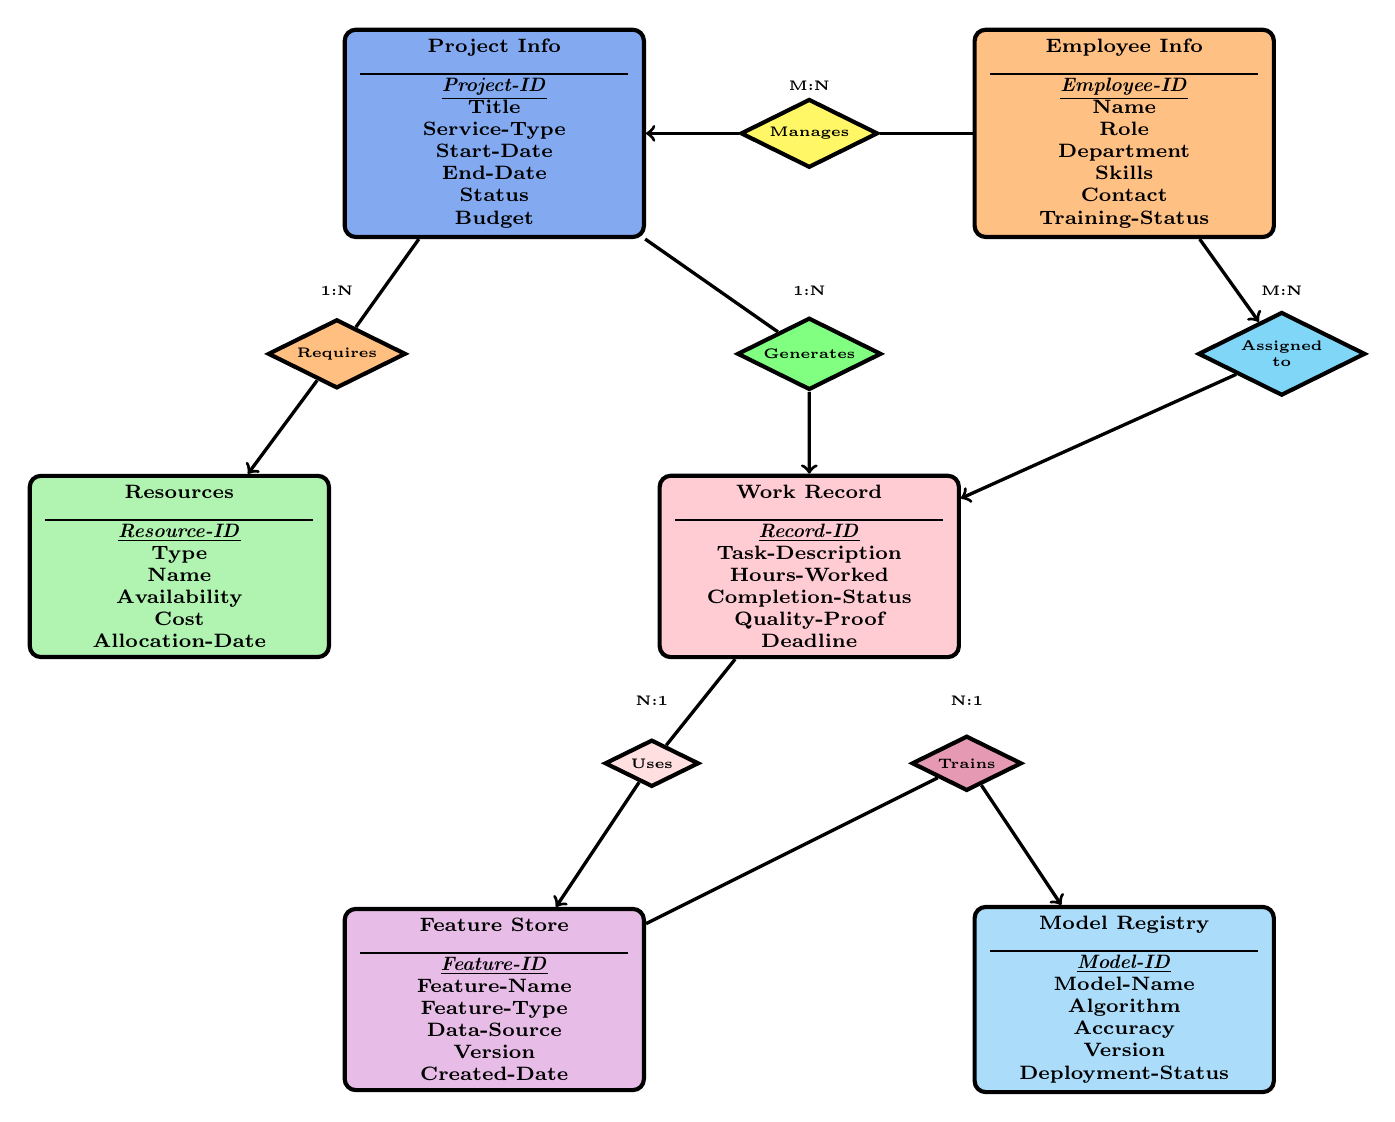
\begin{tikzpicture}[
    entity/.style={rectangle, draw=black, line width=1.5pt, rounded corners, minimum width=3.8cm, minimum height=1.2cm, align=center, font=\scriptsize\bfseries},
    relation/.style={diamond, draw=black, line width=1.5pt, aspect=2, inner sep=2pt, align=center, font=\tiny\bfseries},
    line/.style={very thick, draw=black}
]

% Define entity colors
\definecolor{projectcolor}{RGB}{100,149,237}     % Cornflower Blue
\definecolor{employeecolor}{RGB}{255,165,79}     % Orange
\definecolor{resourcecolor}{RGB}{144,238,144}    % Light Green
\definecolor{workcolor}{RGB}{255,182,193}        % Light Pink
\definecolor{featurecolor}{RGB}{221,160,221}     % Plum
\definecolor{modelcolor}{RGB}{135,206,250}       % Sky Blue

% Top Row - Main Entities
\node[entity, fill=projectcolor!80] (project) at (0,0) {
    \textbf{Project Info}\\\rule{3.4cm}{0.5pt}\\[-2pt]
    \underline{\textit{Project-ID}}\\
    {\scriptsize Title}\\
    {\scriptsize Service-Type}\\
    {\scriptsize Start-Date}\\
    {\scriptsize End-Date}\\
    {\scriptsize Status}\\
    {\scriptsize Budget}
};

\node[entity, fill=employeecolor!70] (employee) at (8,0) {
    \textbf{Employee Info}\\\rule{3.4cm}{0.5pt}\\[-2pt]
    \underline{\textit{Employee-ID}}\\
    {\scriptsize Name}\\
    {\scriptsize Role}\\
    {\scriptsize Department}\\
    {\scriptsize Skills}\\
    {\scriptsize Contact}\\
    {\scriptsize Training-Status}
};

% Middle Row
\node[entity, fill=resourcecolor!70] (resources) at (-4,-5.5) {
    \textbf{Resources}\\\rule{3.4cm}{0.5pt}\\[-2pt]
    \underline{\textit{Resource-ID}}\\
    {\scriptsize Type}\\
    {\scriptsize Name}\\
    {\scriptsize Availability}\\
    {\scriptsize Cost}\\
    {\scriptsize Allocation-Date}
};

\node[entity, fill=workcolor!70] (work) at (4,-5.5) {
    \textbf{Work Record}\\\rule{3.4cm}{0.5pt}\\[-2pt]
    \underline{\textit{Record-ID}}\\
    {\scriptsize Task-Description}\\
    {\scriptsize Hours-Worked}\\
    {\scriptsize Completion-Status}\\
    {\scriptsize Quality-Proof}\\
    {\scriptsize Deadline}
};

% Bottom Row - AI Components
\node[entity, fill=featurecolor!70] (feature) at (0,-11) {
    \textbf{Feature Store}\\\rule{3.4cm}{0.5pt}\\[-2pt]
    \underline{\textit{Feature-ID}}\\
    {\scriptsize Feature-Name}\\
    {\scriptsize Feature-Type}\\
    {\scriptsize Data-Source}\\
    {\scriptsize Version}\\
    {\scriptsize Created-Date}
};

\node[entity, fill=modelcolor!70] (model) at (8,-11) {
    \textbf{Model Registry}\\\rule{3.4cm}{0.5pt}\\[-2pt]
    \underline{\textit{Model-ID}}\\
    {\scriptsize Model-Name}\\
    {\scriptsize Algorithm}\\
    {\scriptsize Accuracy}\\
    {\scriptsize Version}\\
    {\scriptsize Deployment-Status}
};

% Relationships
\node[relation, fill=yellow!60] (manages) at (4,0) {Manages};
\node[relation, fill=orange!50] (requires) at (-2,-2.8) {Requires};
\node[relation, fill=green!50] (generates) at (4,-2.8) {Generates};
\node[relation, fill=cyan!50] (assigned) at (10,-2.8) {Assigned\\to};
\node[relation, fill=pink!50] (uses) at (2,-8) {Uses};
\node[relation, fill=purple!40] (trains) at (6,-8) {Trains};

% Connections
\draw[line, ->] (employee) -- (manages) -- (project);
\draw[line, ->] (project) -- (requires) -- (resources);
\draw[line, ->] (project) -- (generates) -- (work);
\draw[line, ->] (employee) -- (assigned);
\draw[line, ->] (assigned) -- (work);
\draw[line, ->] (work) -- (uses) -- (feature);
\draw[line, ->] (feature) -- (trains) -- (model);

% Cardinalities with colored backgrounds
\node[font=\tiny\bfseries, fill=white, inner sep=1pt] at (4,0.6) {M:N};
\node[font=\tiny\bfseries, fill=white, inner sep=1pt] at (-2,-2) {1:N};
\node[font=\tiny\bfseries, fill=white, inner sep=1pt] at (4,-2) {1:N};
\node[font=\tiny\bfseries, fill=white, inner sep=1pt] at (10,-2) {M:N};
\node[font=\tiny\bfseries, fill=white, inner sep=1pt] at (2,-7.2) {N:1};
\node[font=\tiny\bfseries, fill=white, inner sep=1pt] at (6,-7.2) {N:1};

\end{tikzpicture}
\caption{Entity–Relationship Diagram (ERD) for Tech Rajshahi AI-Powered Project Management System}
\label{fig:erd_diagram}
\end{figure}

The ERD illustrates the six core databases and their relationships within the AI-Powered Project Management and Automation system:

\textbf{Entities and Their Attributes:}
\begin{itemize}
    \item \textbf{Project Info} (Blue): Stores project details including Project-ID, Title, Service-Type, Start-Date, End-Date, Status, and Budget.
    
    \item \textbf{Employee Info} (Orange): Contains employee information including Employee-ID, Name, Role, Department, Skills, Contact, and Training-Status.
    
    \item \textbf{Resources} (Green): Maintains resource data including Resource-ID, Type, Name, Availability, Cost, and Allocation-Date.
    
    \item \textbf{Work Record} (Pink): Tracks work activities with Record-ID, Task-Description, Hours-Worked, Completion-Status, Quality-Proof, and Deadline.
    
    \item \textbf{Feature Store} (Purple): AI component storing Feature-ID, Feature-Name, Feature-Type, Data-Source, Version, and Created-Date.
    
    \item \textbf{Model Registry} (Sky Blue): AI model repository containing Model-ID, Model-Name, Algorithm, Accuracy, Version, and Deployment-Status.
\end{itemize}

\textbf{Relationships:}
\begin{itemize}
    \item \textbf{Employee Manages Project} (M:N): Multiple employees can manage multiple projects, enabling collaborative project management.
    
    \item \textbf{Project Requires Resources} (1:N): Each project requires multiple resources for successful execution.
    
    \item \textbf{Project Generates Work Record} (1:N): A project generates multiple work records tracking various tasks and activities.
    
    \item \textbf{Employee Assigned to Work Record} (M:N): Multiple employees can be assigned to multiple work records, facilitating team collaboration.
    
    \item \textbf{Work Record Uses Feature Store} (N:1): Multiple work records utilize features from the Feature Store for AI-powered analytics.
    
    \item \textbf{Feature Store Trains Model Registry} (N:1): Features are used to train and update AI models in the Model Registry.
\end{itemize}

This database architecture integrates traditional project management data with AI components (Feature Store and Model Registry), enabling intelligent automation, predictive analytics, and data-driven decision-making throughout the project lifecycle.

\newpage
\subsubsection{Software and Technology Stack}
The technology stack for the AI‑Powered Project Management and Automation system has been carefully selected to ensure performance, maintainability, and scalability:

\begin{table}[H]
    \centering
    \renewcommand{\arraystretch}{1.3}
    \begin{tabular}{|p{4cm}|p{10cm}|}
        \hline
        \rowcolor{tableheader}
        \textcolor{headertext}{\textbf{Component}} & \textcolor{headertext}{\textbf{Technology}} \\
        \hline
        Backend Framework & Node.js with Express or Python with Django/Flask \\
        \hline
        Frontend Framework & React.js or Vue.js with Tailwind CSS \\
        \hline
        Database & MySQL or PostgreSQL \\
        \hline
        AI/ML Libraries & TensorFlow, PyTorch, or Scikit‑learn \\
        \hline
        Authentication & OAuth 2.0, JWT (JSON Web Tokens) \\
        \hline
        Cloud Services & AWS, Google Cloud, or Microsoft Azure \\
        \hline
        Version Control & Git with GitHub or GitLab \\
        \hline
        Containerization & Docker \\
        \hline
        CI/CD Pipeline & GitHub Actions or Jenkins \\
        \hline
        Monitoring & Prometheus, Grafana, or New Relic \\
        \hline
    \end{tabular}
    \caption{Technology Stack for Tech Rajshahi's System}
    \label{tab:tech_stack}
\end{table}

\subsubsection{Deployment Environment}
Tech Rajshahi's system will be deployed within a secure, containerized environment for better resource management and faster deployment cycles.  The deployment architecture ensures portability, automation, and fault tolerance through the following technologies and practices:

\begin{itemize}
    \item \textbf{Operating Environment:} A Linux‑based system (preferably Ubuntu Server or CentOS) serves as the host operating system for stability and performance.
    
    \item \textbf{Containerization:} \textit{Docker} containers encapsulate application components, allowing consistent deployment across testing, staging, and production environments.
    
    \item \textbf{Orchestration:} \textit{Docker Compose} or \textit{Kubernetes} is used to manage container clusters, handle load balancing, and automate scaling based on traffic and workload.
    
    \item \textbf{CI/CD Pipelines:} Continuous Integration and Continuous Deployment pipelines are implemented using \textit{GitHub Actions} or \textit{Jenkins}.  These pipelines automate code testing, building, and deployment, significantly reducing downtime and manual errors.
    
    \item \textbf{Version Control and Rollback:} The system supports versioned deployments with rollback capabilities, ensuring operational continuity in case of system errors or bugs introduced in new releases.
\end{itemize}

This deployment strategy ensures that updates, patches, and new features can be rolled out rapidly and securely without disrupting ongoing operations.

\subsection{Functional Decomposition and Structured Chart}
A \textbf{Structured Chart} is a hierarchical diagram that represents the modular design of a system by breaking down complex functions into smaller, manageable components.  It illustrates the functional decomposition of the system, showing how high‑level processes are subdivided into lower‑level modules, and depicts the relationships, control flow, and data flow between these modules.  For Tech Rajshahi's AI‑Powered Project Management and Automation system, the structured chart provides a clear visualization of the system's architecture, demonstrating how different functional units interact to deliver the complete solution.

The functional decomposition follows a top‑down approach, systematically breaking down the system from the most abstract level (Level~0) to increasingly detailed levels (Level~1, Level~2, and Level~3), ensuring comprehensive coverage of all system functionalities.

\subsubsection{Level 0: System Overview}
At \textbf{Level~0}, the system is represented as a single high‑level module: the \textit{Proposed Tech Rajshahi System}.  This represents the entire system as a unified entity responsible for managing all organizational activities.  The system receives inputs including \textit{Client Inquiries}, \textit{Client Feedback and Requirements}, \textit{Operational Service Request}, and \textit{Project Deliverables Requirements}, and produces outputs including \textit{Financial Summary Report}, \textit{Project Deliverables Requirements}, \textit{Departmental Setup Report}, \textit{Support Result}, and \textit{Completed Project Records}.  Level~0 establishes the system's boundary and defines its primary purpose without revealing internal structure.

\subsubsection{Level 1: Major Functional Modules}
\textbf{Level~1} decomposes the top‑level system into five major functional modules, each representing a distinct area of responsibility:

\begin{itemize}
    \item \textbf{Financial Management:} Manages all financial operations including transactions, reporting, budgeting, and billing activities.  It receives \textit{Payment Processing Request} as input and produces \textit{Report Output}, \textit{Budget Plan}, and \textit{Financial Analysis Result} as outputs.
    
    \item \textbf{Client Relationship Management:} Handles all client‑related interactions, requirements gathering, contract management, and payment processing.  It receives \textit{Client Inquiries}, \textit{Approved Response}, \textit{Payment Record}, and \textit{Job Offers} as inputs, and produces \textit{Client Request and Query Management} output.
    
    \item \textbf{Human Resource Management:} Manages employee recruitment, talent retention, training, performance evaluation, and employee data.  It receives \textit{Job Offers}, \textit{Training Performance}, and \textit{Employee Input Data} as inputs, and produces \textit{Selected Candidate Details} and \textit{Employee Details} as outputs.
    
    \item \textbf{Departmental Services Management:} Coordinates development services across different departments and manages the AI‑powered task scheduling system.  It receives \textit{Departmental Setup Data} as input and produces \textit{Departmental Setup Report} and \textit{Development Team Report} as outputs.
    
    \item \textbf{Product Delivery Management:} Oversees the entire product delivery lifecycle including quality assurance, customer support, and final project delivery.  It receives \textit{Support Request}, \textit{Quality Approval Result}, \textit{Delivery Confirmation}, and \textit{Client Feedback} as inputs, and produces \textit{Support Summary Report}, \textit{UI/UX Development Team Report}, \textit{Customer Feedbacks Product Related}, and \textit{Financial Support Reports} as outputs.
\end{itemize}

These Level~1 modules represent the primary functional divisions of the system, each encapsulating a specific domain of business logic while maintaining clear interfaces for inter‑module communication.

\subsubsection{Level 2: Sub-Module Decomposition}
\textbf{Level~2} further decomposes each Level~1 module into specialized sub‑modules that handle specific functionalities within their parent module:

\begin{itemize}
    \item \textbf{Financial Management} breaks down into:
    \begin{itemize}
        \item \textit{Transactions Management:} Handles payment processing and transaction records
        \item \textit{Financial Reports Generation:} Produces financial analysis reports and variance reports
        \item \textit{Budget Planning and Management:} Manages budget preparation and cost adjustments
    \end{itemize}
    
    \item \textbf{Client Relationship Management} subdivides into:
    \begin{itemize}
        \item \textit{Request and Query Management:} Processes client inquiries and manages responses
        \item \textit{Contract and Agreement Management:} Handles contract approvals and agreements
        \item \textit{Payment and Billings:} Manages payment records and billing processes
    \end{itemize}
    
    \item \textbf{Human Resource Management} contains:
    \begin{itemize}
        \item \textit{Recruitment:} Manages job offers and candidate selection processes
        \item \textit{Talent Retention:} Handles employee engagement and retention strategies
        \item \textit{AI Powered Lifecycle Scheduling:} Implements AI‑based task and lifecycle scheduling
    \end{itemize}
    
    \item \textbf{Departmental Services Management} includes:
    \begin{itemize}
        \item \textit{Development Services:} Coordinates web development, app development, and other development activities
    \end{itemize}
    
    \item \textbf{Product Delivery Management} comprises:
    \begin{itemize}
        \item \textit{Support Services:} Provides customer support and feedback management
        \item \textit{Quality Assurance:} Ensures product quality through testing and validation
        \item \textit{Customer Review:} Collects and processes customer feedback and reviews
        \item \textit{Project Delivery:} Manages final project delivery and handover
    \end{itemize}
\end{itemize}

At this level, the decomposition reveals the internal structure of each major module, showing how complex functionalities are divided into cohesive, manageable units that can be developed, tested, and maintained independently.

\subsubsection{Level 3: Detailed Component Functions}
\textbf{Level~3} represents the most granular decomposition, breaking down Level~2 sub‑modules into atomic functional components that perform specific, well‑defined operations.  These are the fundamental building blocks of the system:

\begin{itemize}
    \item \textbf{Financial Management} Level~3 components include:
    \begin{itemize}
        \item \textit{Daily and Monthly Transaction Statements:} Generates detailed transaction records
        \item \textit{Budget Variance Analysis:} Analyzes budget deviations and variances
        \item \textit{Budget Preparation:} Prepares organizational budgets
        \item \textit{Cost:} Manages cost tracking and analysis
        \item \textit{Financial Analysis:} Performs comprehensive financial analysis
    \end{itemize}
    
    \item \textbf{Client Relationship Management} Level~3 components include:
    \begin{itemize}
        \item \textit{Skill Gap Analysis:} Identifies skill gaps in client requirements
        \item \textit{Training Employee:} Coordinates training for client‑facing employees
        \item \textit{Fair Assignment of Tasks:} Ensures equitable task distribution
    \end{itemize}
    
    \item \textbf{Departmental Services Management} Level~3 components include:
    \begin{itemize}
        \item \textit{Web Development:} Manages web development projects
        \item \textit{App Development:} Handles mobile and application development
        \item \textit{UI/UX Development:} Oversees user interface and experience design
    \end{itemize}
    
    \item \textbf{Product Delivery Management} Level~3 components include:
    \begin{itemize}
        \item \textit{Customer Feedbacks Product Related Support:} Processes product‑related customer feedback
        \item \textit{Financial Supports:} Manages financial support documentation
    \end{itemize}
\end{itemize}

Level~3 components represent individual functions or procedures that can be directly implemented as methods, classes, or microservices in the actual codebase.  Each component has clearly defined inputs, outputs, processing logic, and interaction patterns with other components.

\subsubsection{Structured Chart Representation}
Figure~\ref{fig:system_architecture} presents the structured chart for the AI‑Powered Project Management and Automation system, visually depicting the hierarchical decomposition from Level~0 through Level~3.  The chart uses standard notations: rectangles represent modules and components, connecting lines indicate control flow and module invocation relationships, and data flow arrows (with labels) show information exchange between modules.

\begin{figure}[H]
    \centering
    \includegraphics[width=\textwidth]{Fig/Structured_Chart.png}
    \caption{Structured Chart of AI‑Powered Project Management System}
    \label{fig:system_architecture}
\end{figure}

The structured chart demonstrates how the main system controller coordinates between different modules, ensuring proper data flow and functional integration while maintaining modularity and maintainability.  The hierarchical structure facilitates understanding of system complexity, supports parallel development by multiple teams, enables independent testing of components, and provides a clear roadmap for implementation.  By following this structured decomposition, Tech Rajshahi ensures that the system architecture is scalable, maintainable, and aligned with software engineering best practices.

\subsection{Coupling and Cohesion}
In software design, \textbf{coupling} and \textbf{cohesion} are essential principles that determine the quality and maintainability of the system.

\subsubsection{Coupling}
Coupling refers to the degree of interdependence between software modules.  \textbf{Loose coupling} is desirable as it allows modules to be modified independently without affecting others.  Tech Rajshahi's system design achieves loose coupling through:
\begin{itemize}
    \item Well‑defined APIs between modules.
    \item Use of message queues for asynchronous communication.
    \item Dependency injection patterns.
    \item Standardized data formats (JSON) for inter‑module communication.
\end{itemize}

\subsubsection{Cohesion}
Cohesion refers to how closely the responsibilities of a single module are related.  \textbf{High cohesion} is desirable as it ensures that each module has a clear, focused purpose.  The system design achieves high cohesion by:
\begin{itemize}
    \item Organizing modules around specific business functions (e.g., Project Management, Billing, AI Analytics).
    \item Ensuring each module handles only related tasks and data.
    \item Following the single responsibility principle.
    \item Minimizing module size and complexity.
\end{itemize}

By maintaining loose coupling and high cohesion, the system becomes more maintainable, testable, and scalable.

\subsection{Design Deliverables}
The system design phase produces several key deliverables that guide the implementation phase:

\begin{itemize}
    \item \textbf{System Architecture Document:} Comprehensive documentation of the system architecture, including diagrams, technology stack, and infrastructure specifications.
    
    \item \textbf{Database Design Document:} Detailed database schema with ER diagrams, table structures, relationships, and data dictionary.
    
    \item \textbf{Interface Specifications:} Wireframes, mockups, and detailed specifications for all user interfaces and navigation flows.
    
    \item \textbf{Security Specifications:} Detailed documentation of security requirements, authentication mechanisms, encryption standards, and access control policies.
    
    \item \textbf{Technical Specifications:} Detailed technical documentation including API specifications, module interfaces, data formats, and integration protocols.
    
    \item \textbf{Test Plans:} Comprehensive test plans covering unit testing, integration testing, performance testing, and user acceptance testing criteria.
\end{itemize}

\subsection{Conclusion}
The system design phase translates the analytical framework established in previous chapters into a practical and well‑structured blueprint for Tech Rajshahi's AI‑Powered Project Management and Automation system.  The logical design ensures modular functionality, data consistency, and smooth integration across departments, while the physical design focuses on performance, scalability, and secure infrastructure.  

Together, these design elements create a foundation that supports efficient project coordination, automated task assignment, intelligent resource allocation, streamlined billing, unified communication, and continuous feedback management.  The multi‑layered security framework ensures data protection and regulatory compliance, while the hybrid infrastructure provides flexibility and reliability.

By adopting a structured yet adaptable design approach, Tech Rajshahi Ltd. is well‑positioned to deploy a future‑ready system that promotes operational excellence, enhances decision‑making capabilities, reduces manual workload, and drives long‑term strategic growth.  The comprehensive design verification process ensures that the system will meet user expectations and business objectives, setting the stage for successful implementation and adoption across the organization.

\end{document}
